\chapter {Syntax and semantics}

The proposal for extending SBML to carry the information for multistate multicomponent species relies on the extension of the following core SBML elements: \class{Species}, \class{InitialAssignment}, \class{Rule}, \class{Reaction}, \class{SimpleSpeciesReference}, \class{EventAssignment}. In addition, the multistate multi-component package requires the creation of new main elements: \class{SpeciesType}, \class{Selector}. 

A software that does not understand \multiVone can ignore entirely all elements in the corresponding namespace. The remaining SBML model is a valid \sbmlLthreeVone core.

In the UML diagrams contained in this specification, the elements and attributes specific to the package \emph{multi} are drawn in red, while the elements and attributes belonging to SBML core are drawn in black. Not all of the latter are drawn, but only the ones needed to "plug" the package \emph{multi}. Please consult the specification of the core for a deeper understanding of SBML at large.
 
\section{Extension of the model element}

In order to encode the structures needed to define and use multistate and multi-component complexes, the element \class{model} is extended to be linked to a list of \class{SpeciesType}s and a list of \class{Selector}s.

\begin{figure}[H]
\begin{center}
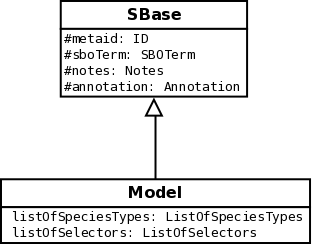
\includegraphics[scale=0.3]{figs/pngs/ModelClass.png} 
\caption{Definition of \class{Model} and its relation with \class{SBase}.}
\label{fig:Model}
\end{center}
\end{figure}

\begin{example}
<model xmlns:multi="http://www.sbml.org/sbml/level3/version1/multi/version1">
  <!-- some compartments -->
  <multi:listOfSpeciesTypes>
    <!-- some species types -->
  </multi:listOfSpeciesTypes>
  <multi:listOfSelectors>
    <!-- some selectors -->
  </multi:listOfSelectors>
  <!-- some species, initialAssignments, rules,  reactions, events -->
</model>
\end{example}
\section{Definition of the species types and their state features}

In order to build multi-component multistate entities, one needs to define the building blocks that will be combined. A given type of component, a \class{SpeciesType},  can carry several \class{StateFeature}s, which are multi-valued characteristics of the component. One can also specify if instances of a \class{SpeciesType} can act as binding sites. Apart from a unique identifier, a name, and several annotations, it is furthermore possible to define state features of a component, and the values taken by those state features.  The following UML diagram shows how the structure of the \class{SpeciesType} looks like. 

\begin{figure}[H]
\begin{center}
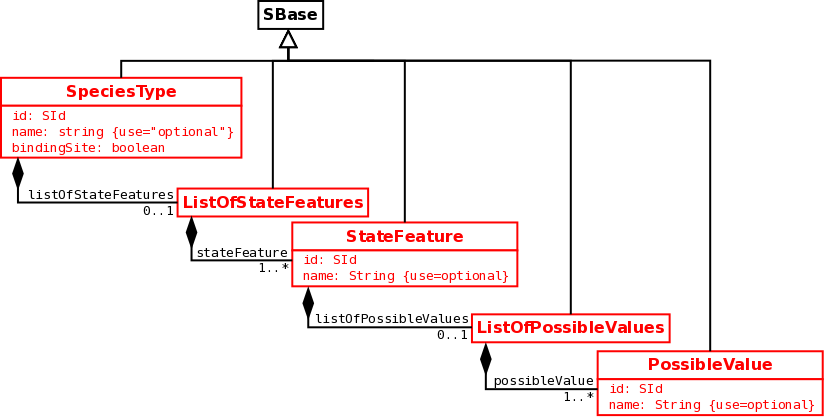
\includegraphics[scale=0.3]{figs/pngs/SpeciesTypeGeneral.png} 
\caption{\class{SpeciesType} and all the associated classes.}
\label{fig:SpeciesTypeGeneral}
\end{center}
\end{figure}

\subsection{SpeciesType} 

The element \class{SpeciesType}, which is part of \sbmlLtwoVfour specification, is not part of \sbmlLthreeVone any more. Instead, it will be defined in the \emph{multi} package. The \class{SpeciesType} element carries not only the basic attributes which it had in \sbmlLtwoVfour (\attribute{metaid}, \attribute{id}, \attribute{name}), but is also extended for the needs of describing multi-component entities with the attribute \attribute{bindingSite} and for the needs of multistate entities by linking it to a list of  \class{StateFeature}s.

\begin{figure}[H]
\begin{center}
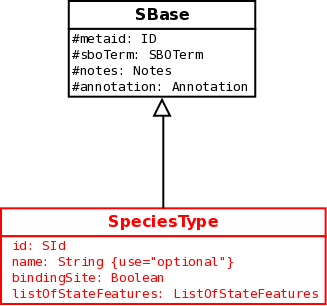
\includegraphics[scale=0.3]{figs/pngs/SpeciesTypeClass.png} 
\caption{Definition of \class{SpeciesType} and its relation with \class{SBase}.}
\label{fig:SpeciesTypeClass}
\end{center}
\end{figure}

A species type can be used to describe a component of a supra-macromolecular assembly, but also a domain of a macromolecule. Such a domain can be a portion of the macromolecule, a non-connex set of atoms forming a functional domain, or just a conceptual construct suiting the needs of the modeler. The type of component can be specified by referring terms from the subbranch \emph{functional entity} of the Systems Biology Ontology (\url{http://biomodels.net/sbo/}, \citep{Lenov:2007}) through the optional \attribute{sboTerm} attribute. The following table provides typical examples of component or domains (the list is absolutely not complete).\\

\begin{center}
\begin{tabular}{ll}
\hline
SBO identifier & definition \\
\hline
SBO:0000242 & channel \\
SBO:0000244 & receptor \\
SBO:0000284 & transporter \\
SBO:0000280 & ligand \\ 
SBO:0000493 & functional domain \\
SBO:0000494 & binding site \\
SBO:0000495 & catalytic site \\
SBO:0000496 & transmembrane domain \\
\hline
\end{tabular}\\[\baselineskip]
\end{center}

The example below encodes a species type representing a ligand-gated ion channel, that is a transmembrane macromolecule that can form a ionic channel stabilised by the binding of ligands. Notice the notes and annotation that belong to the namespace of \sbmlLthreeVone \emph{core}.

\begin{example}
<multi:speciesType xmlns:core="http://www.sbml.org/sbml/level3/version1"
                   xmlns:multi="http://www.sbml.org/sbml/level3/version1/multi/version1" 
                   xmlns:xhtml="http://www.w3.org/1999/xhtml"
                   xmlns:rdf="http://www.w3.org/1999/02/22-rdf-syntax-ns#" 
                   xmlns:bqbiol="http://biomodels.net/biology-qualifiers/"
                   multi:id="speciesType1"
                   multi:name="LGIC"
                   multi:bindingSite="false" 
                   multi:sboTerm="SBO:0000242">
  <core:notes>
    <xhtml:body>
      <xhtml:p>LGIC is a Ligand-Gated Ion Channel</xhtml:p>
    </xhtml:body>
  </core:notes>
  <core:annotation>
    <rdf:RDF>
      <rdf:Description rdf:about="#_000003">
        <bqbiol:isVersionOf>
          <rdf:Bag>
            <rdf:li rdf:resource="urn:miriam:interpro:IPR002394"/>
          </rdf:Bag>
        </bqbiol:isVersionOf>
      </rdf:Description>
    </rdf:RDF>
  </core:annotation>
  <multi:listOfStateFeatures>
    <!-- some state features -->
  </multi:listOfStateFeatures>
</multi:speciesType>
\end{example}

The example below encodes a species type representing the binding site for a ligand, that could be used for instance in conjunction with the previous example. 

\begin{example}
<multi:speciesType xmlns:multi="http://www.sbml.org/sbml/level3/version1/multi/version1" 
                   multi:id="speciesType2"
                   multi:name="AgonistSite" 
                   multi:bindingSite="true" 
                   multi:sboTerm="SBO:0000494" />
\end{example}

\subsection{StateFeature} 

A species type can carry any number of state features, which are characteristic properties specific for this type of species. The element \class{StateFeature} of \sbmlLthreeVone \multiVone corresponds to the ``state variable'' of the SBGN Entity Relationship language. A \class{StateFeature} is identified by an \attribute{id} and an optional \attribute{name}. A \class{StateFeature} is linked to a list of \class{PossibleValue}s.

\begin{figure}[H]
\begin{center}
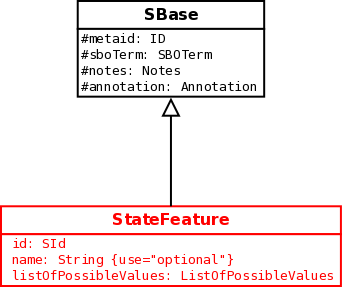
\includegraphics[scale=0.3]{figs/pngs/StateFeatureClass.png} 
\caption{Definition of \class{StateFeatureClass} and its relation with \class{SBase}.}
\label{fig:StateFeatureClass}
\end{center}
\end{figure}

As all elements derived from \class{SBase}, \class{StateFeature} can link to \class{Notes} and \class{Annotation}, and carry a \attribute{metaid}, and an \attribute{sboTerm}. The value \cdata{SBO:0000497} of \attribute{sboTerm} used in the example below corresponds to a ``ternary switch''.

%% Add notes and annotations below
\begin{example}
<multi:stateFeature 
              xmlns:multi="http://www.sbml.org/sbml/level3/version1/multi/version1" 
              multi:id="stateFeature1"
              multi:name="pore"
              multi:sboTerm="SBO:0000497">
  <multi:listOfPossibleValues>
    <!-- some possible values -->
  </multi:listOfPossibleValues>
</multi:stateFeature>
\end{example}

\subsection{PossibleValue}

Each state feature also requires the definition of all the possible values it can take. Those values will be used within a selector, to define the states an entity is allowed to take. A state feature is not obligatory a boolean property, but can carry any number of \class{PossibleValue}. A \class{PossibleValue} is identified by an \attribute{id} and an optional \attribute{name}.

\begin{figure}[H]
\begin{center}
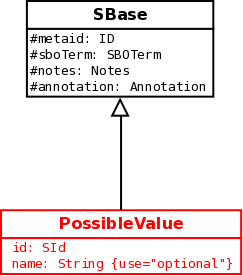
\includegraphics[scale=0.3]{figs/pngs/PossibleValueClass.png} 
\caption{Definition of \class{PossibleValue} and its relation with \class{SBase}.}
\label{fig:PossibleValueClass}
\end{center}
\end{figure}

As all elements derived from \class{SBase}, \class{PossibleValue} can link to \class{Notes} and \class{Annotation}, and carry a \attribute{metaid}, and an \attribute{sboTerm}. The \attribute{sboTerm} used in the example below corresponds to a ``ternary switch''. 

\begin{example}
<multi:possibleValue 
                     xmlns:multi="http://www.sbml.org/sbml/level3/version1/multi/version1" 
                     multi:id="possibleValue1" 
                     multi:name="open"
                     multi:sboTerm="0000416" />
\end{example}

\subsection{Complete definition of a species type}

The following example describes the SpeciesType presented on \fig{st_receptor}.

\begin{example}
<multi:speciesType xmlns:core="http://www.sbml.org/sbml/level3/version1"
                   xmlns:multi="http://www.sbml.org/sbml/level3/version1/multi/version1" 
                   xmlns:xhtml="http://www.w3.org/1999/xhtml"
                   xmlns:rdf="http://www.w3.org/1999/02/22-rdf-syntax-ns#" 
                   xmlns:bqbiol="http://biomodels.net/biology-qualifiers/"
                   multi:id="speciesType1"
                   multi:bindingSite="false" 
                   multi:name="LGIC" 
                   multi:sboTerm="SBO:0000242">
  <core:notes>
    <xhtml:body>
      <xhtml:p> 
        LGIC is a Ligand-Gated Ion Channel. It contains a pore that can be open or closed.
      </xhtml:p>
    </xhtml:body>
  </core:notes>
  <core:annotation>
    <rdf:RDF>
      <rdf:Description rdf:about="#_000003">
        <bqbiol:isVersionOf>
          <rdf:Bag>
            <rdf:li rdf:resource="urn:miriam:interpro:IPR002394"/>
          </rdf:Bag>
        </bqbiol:isVersionOf>
      </rdf:Description>
    </rdf:RDF>
  </core:annotation>
  <multi:listOfStateFeatures>
    <multi:stateFeature multi:id="stateFeature1"
                        multi:name="pore"
                        multi:sboTerm="SBO:0000497">
      <multi:listOfPossibleValues>
        <multi:possibleValue id="possibleValue1"
                             multi:name="open"
                             multi:sboTerm="SBO:0000416" />
        <multi:possibleValue id="possibleValue2"
                             multi:name="closed"
                             multi:sboTerm="SBO:0000417" />
        <multi:possibleValue id="possibleValue3"
                             multi:name="desensitised"
                             multi:sboTerm="SBO:0000417" />
      </multi:listOfPossibleValues>
    </multi:stateFeature>
  </multi:listOfStateFeatures>
</multi:speciesType>
\end{example}

\section{Definition of filters to select states and topologies }
 
A selector is a mask describing the rules that an entity has to pass in order to be used or rejected. This selector is built of different components, carrying state features. The components can be bound together or not. In a population-based model, the selector, when applied to a pool of entities, permits to filter it, and to obtain a further, more refined, entity pool.

\begin{figure}[H]
\begin{center}
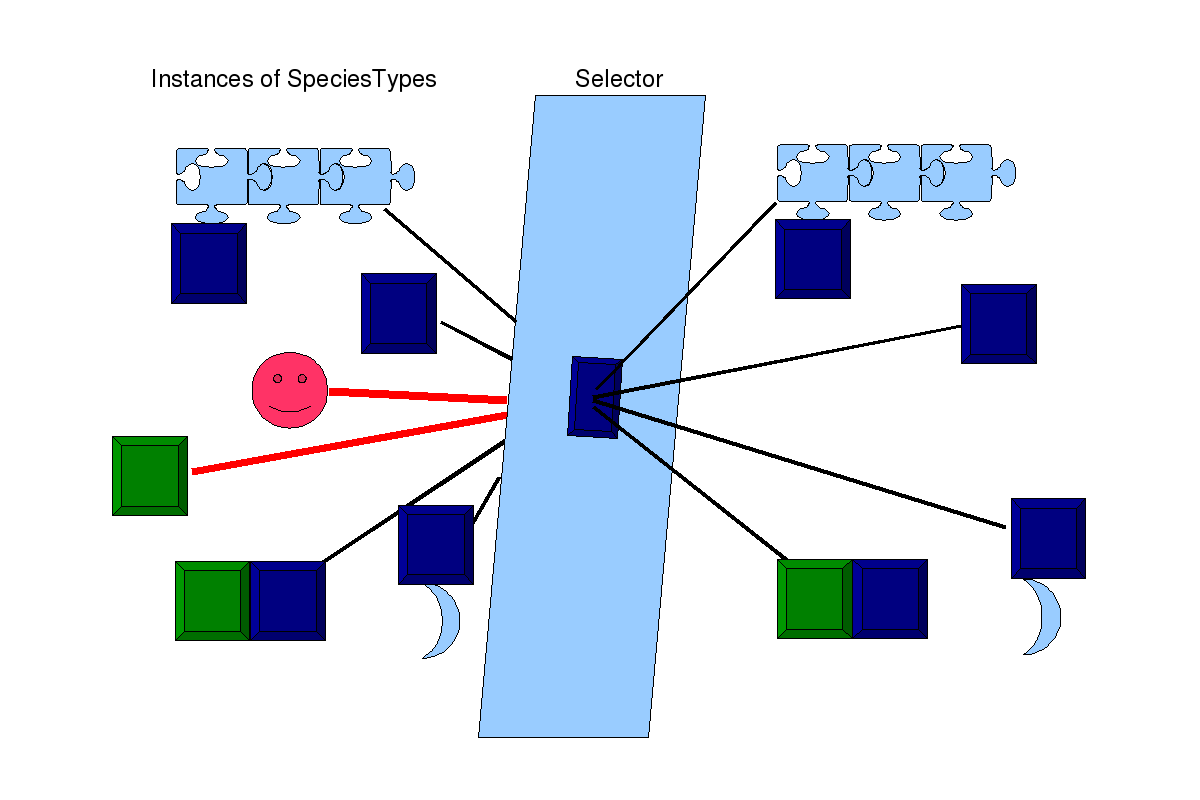
\includegraphics[scale=0.3]{figs/pngs/PrincipleIdeaSelector.png} 
\caption{The above selector accepts everything containing a blue crystal, but rejects the red face and the isolated green crystal.}
\label{fig:PrincipleIdeaSelector}
\end{center}
\end{figure}

A selector can be reused in various places of a model, to restrict the application of a procedure to a certain set of topologies and states. Selectors can be used to refine the initial conditions of a species, for instance to specify the initial distribution of different states and topologies. They can also be used in a reaction to decide if a this reaction happens, or to modulate its velocity, in function of the state or topology of a reactant. 

A selector defines the list of components composing the mask, that are species type existing under a given state (that can be an ensemble of elementary states). In addition to the components, the selector lists the possible or mandatory bonds, as well as the components that must not be bound. It is to be noted that a selector must not necessarily be the most parsimonious. One can use the selectors to describe the fine-grained topology of complexes, even if this topology is not used to decide upon particular reactions. The general structure of the selector is provided in \fig{SelectorGeneral} and the general structure of the species type state is provided in \fig{SpeciesTypeStateGeneral}.

\begin{figure}[H]
\begin{center}
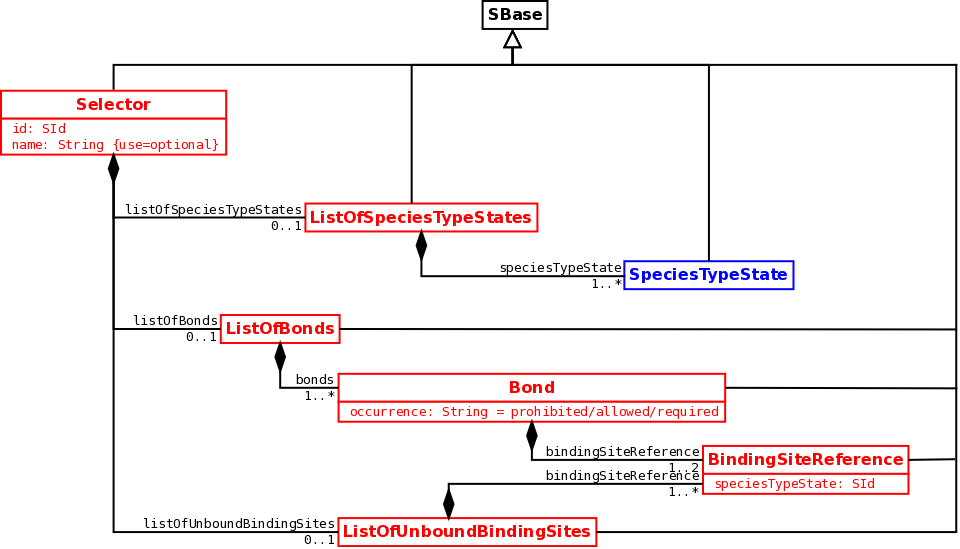
\includegraphics[scale=0.3]{figs/pngs/SelectorGeneral.png} 
\caption{\class{Selector} and all the associated classes.}
\label{fig:SelectorGeneral}
\end{center}
\end{figure}


\begin{figure}[H]
\begin{center}
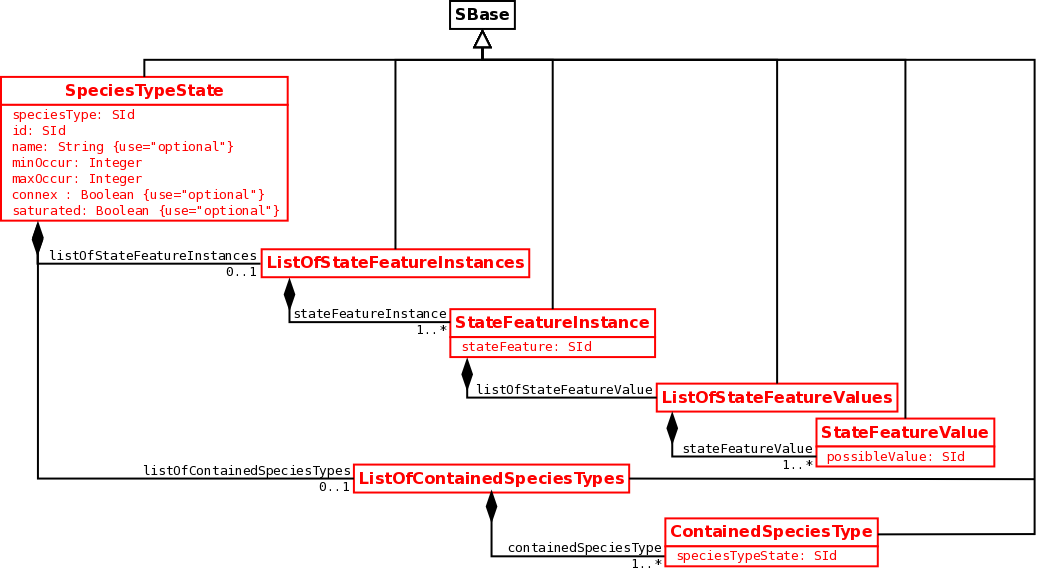
\includegraphics[scale=0.25]{figs/pngs/SpeciesTypeStateGeneral.png} 
\caption{\class{SpeciesTypeState} and all the associated classes.}
\label{fig:SpeciesTypeStateGeneral}
\end{center}
\end{figure}

A graphical representation of how to build a selector to encode a complex entity is represented on \fig{selectorBuilding}.

\begin{figure}[H]
\begin{center}
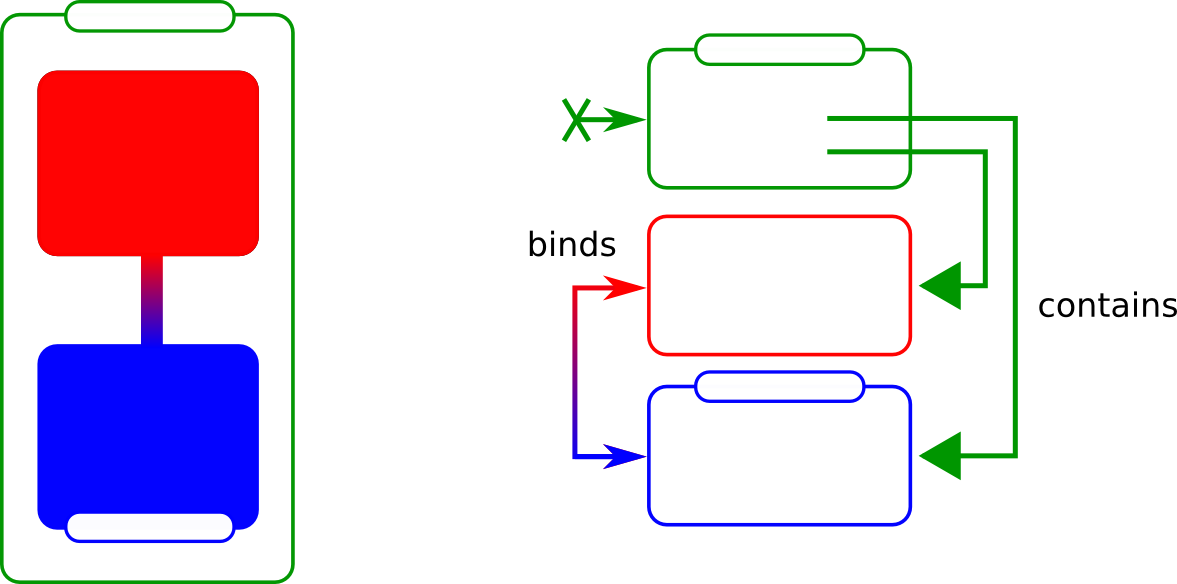
\includegraphics[scale=0.5]{figs/pngs/selectorBuilding.png}
\caption{This figure illustrates the procedure by which a selector builds the representation of a multi-state, multi-component complex. To encode the left part, representing the complex following the conventions used in this document, we write part represented on the right, listing the different components and their relationships.}
\label{fig:selectorBuilding}
\end{center}
\end{figure}

The \attribute{id} of \class{SpeciesTypeState} belong to a namespace local to the containing selector. Therefore, one can use the same values for \attribute{id} of \class{SpeciesTypeState} in different selectors. However, within a selector, all the values for \attribute{id} of \class{SpeciesTypeState} must be different.

\subsection{Selector}

A \class{Selector} is identified by an \attribute{id} and an optional \attribute{name}. As all elements derived from \class{SBase}, it can link to \class{Notes} and \class{Annotation}, and carry a \attribute{metaid}, and an \attribute{sboTerm}. In addition, a \class{Selector} is linked to a list of \class{SpeciesTypeState}s, a list of \class{Bond}s and  a list of  \class{BindingSiteReference}s.

\begin{figure}[H]
\begin{center}
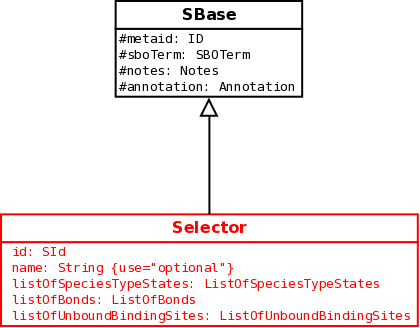
\includegraphics[scale=0.3]{figs/pngs/SelectorClass.png} 
\caption{Definition of \class{Selector} and its relation with \class{SBase}.}
\label{fig:SelectorClass}
\end{center}
\end{figure}

\begin{example}
<multi:selector 
                xmlns:multi="http://www.sbml.org/sbml/level3/version1/multi/version1" 
                multi:id="selector1"
                multi:name="unbound_receptor">
  <multi:listOfSpeciesTypeStates>
    <!-- some species type state -->
  </multi:listOfSpeciesTypeStates>
  <multi:listOfBonds>
    <!-- some bonds -->
  </multi:listOfBonds>
  <multi:listOfUnboundBindingSites>
    <!-- some unbound binding sites -->
  </multi:listOfUnboundBindingSites>
</multi:selector>
\end{example}

\subsection{SpeciesTypeState}

A species type state describes an ensemble of instances of a species type can be into, in order to fulfill the requirements of the selector. In order to build complex multi-component species, an instance of a species type can contain other instances of species types, that have to be declared in the selector also, with their allowed states. A species type state is then defined by the values of the different state features carried by the species type, the list of species type states it "contains", and their topology.
A \class{SpeciesTypeState} is identified by an \attribute{id} and an optional \attribute{name} plus an attribute \attribute{speciesType}, pointing to the \class{SpeciesType} it instantiates. As all elements derived from \class{SBase}, it can link to \class{Notes} and \class{Annotation}, and carry a \attribute{metaid}, and an \attribute{sboTerm}. In addition, a \class{SpeciesTypeState} can be linked to a list of \class{StateFeatureInstance}s and a list of \class{ContainedSpeciesType}s. A \class{SpeciesTypeState} can be instantiated several times in a selector, using the attributes \attribute{minOccur} and \attribute{maxOccur}. The attribute \attribute{connex} precises that all those instances must be part of a continuous network through bonds formed by the \class{ContainedSpeciesType}s. The attribute \attribute{saturated} precises that all \class{ContainedSpeciesType}s that are instances of \class{SpeciesType} with their attribute \attribute{bindingSite} set to true must be involved in bonds. 

\begin{figure}[H]
\begin{center}
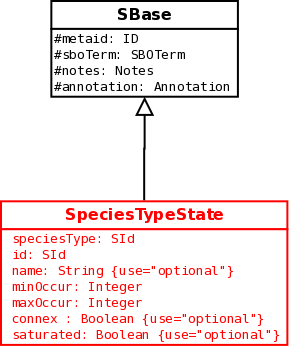
\includegraphics[scale=0.3]{figs/pngs/SpeciesTypeStateClass.png} 
\caption{Definition of \class{SpeciesTypeState} and its relation with \class{SBase}.}
\label{fig:SpeciesTypeStateClass}
\end{center}
\end{figure}

\begin{example}
<multi:speciesTypeState 
                    xmlns:multi="http://www.sbml.org/sbml/level3/version1/multi/version1" 
                    multi:id="speciesTypeState1" multi:name="open_receptor"
                    multi:speciesType="speciesType1"
                    multi:minOccur="2" multi:maxOccur="4"
                    multi:connex="true" multi:saturated="true" >
  <multi:listOfStateFeatureInstances>
    <!-- some state feature instances -->
  </multi:listOfStateFeatureInstances>
  <multi:listOfContainedSpeciesTypes>
    <!-- some contained species types -->
  </multi:listOfContainedSpeciesTypes>
</multi:speciesTypeState>
\end{example}

\subsection{StateFeatureInstance}

The possible states of an instance of species type are described using the state features of that species type. Only the meaningful state features, that are used to specified the state, must be listed. The other are assumed to take any value, to be wildcards. A  \class{StateFeatureInstance} is identified by an attribute \attribute{StateFeature}, pointing to the \class{StateFeature} it instantiates. As all elements derived from \class{SBase}, it can link to \class{Notes} and \class{Annotation}, and carry a \attribute{metaid}, and an \attribute{sboTerm}. In addition, a \class{StateFeatureInstance} can be linked to a list of \class{StateFeatureValue}s.

\begin{figure}[H]
\begin{center}
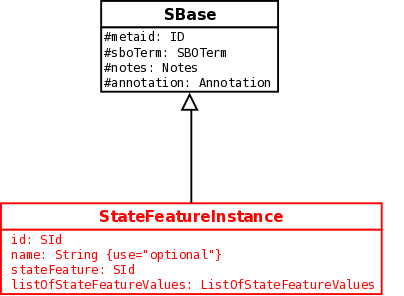
\includegraphics[scale=0.5]{figs/pngs/StateFeatureInstanceClass.png} 
\caption{Definition of \class{StateFeatureInstance} and its relation with \class{SBase}.}
\label{fig:StateFeatureInstanceClass}
\end{center}
\end{figure}

\begin{example}
<multi:stateFeatureInstance 
                    xmlns:multi="http://www.sbml.org/sbml/level3/version1/multi/version1" 
                    multi:stateFeature="stateFeature1">
  <!-- some state feature values -->
</multi:stateFeatureInstance>
\end{example}

\subsection{StateFeatureValue}

The selector specifies the values that a state feature of an instance of species type can take. A  \class{StateFeatureValue} points to the relevant \class{PossibleValue}s defined in the instantiated \class{SpeciesTypes} using an attribute \attribute{possibleValue}. As all elements derived from \class{SBase}, \class{StateFeatureValue} can link to \class{Notes} and \class{Annotation}, and carry a \attribute{metaid}, and an \attribute{sboTerm}.

\begin{figure}[H]
\begin{center}
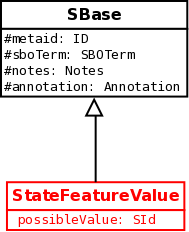
\includegraphics[scale=0.3]{figs/pngs/StateFeatureValueClass.png} 
\caption{Definition of \class{StateFeatureValue} and its relation with \class{SBase}.}
\label{fig:StateFeatureValueClass}
\end{center}
\end{figure}

\begin{example}
<multi:stateFeatureValue 
                    xmlns:multi="http://www.sbml.org/sbml/level3/version1/multi/version1" 
                    multi:possibleValue="possibleValue1" />
\end{example}

\subsection{ContainedSpeciesType}

In order to build complex nested multi-component species, an instance of a species type can contain other instances of species types, that have to be declared in the same selector. As all elements derived from \class{SBase}, \class{ContainedSpeciesType} can link to \class{Notes} and \class{Annotation}, and carry a \attribute{metaid}, and an \attribute{sboTerm}. In addition, a \class{ContainedSpeciesType} points to the relevant \class{SpeciesTypeState} using an attribute \attribute{speciesTypeState}. 

\begin{figure}[H]
\begin{center}
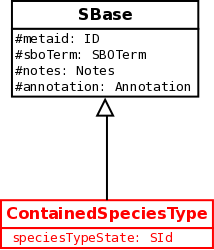
\includegraphics[scale=0.3]{figs/pngs/ContainedSpeciesTypeClass.png} 
\caption{Definition of \class{ContainedSpeciesType} and its relation with \class{SBase}.}
\label{fig:ContainedSpeciesTypeClass}
\end{center}
\end{figure}

\begin{example}
<multi:containedSpeciesType 
             xmlns:multi="http://www.sbml.org/sbml/level3/version1/multi/version1" 
             multi:speciesTypeState="speciesType1" />
\end{example}

\subsection{Bond}

The connectivity between the components of a selector is described by listing the bonds that are possible, mandatory or forbidden. As all elements derived from \class{SBase}, \class{Bond} can link to \class{Notes} and \class{Annotation}, and carry a \attribute{metaid}, and an \attribute{sboTerm}. An attribute \attribute{occurrence} specifies if a bond is \cdata{required}, \cdata{allowed} or \cdata{prohibited}. In addition, a \class{Bond} can be linked to a one or two \class{BindingReference}s.

\begin{figure}[H]
\begin{center}
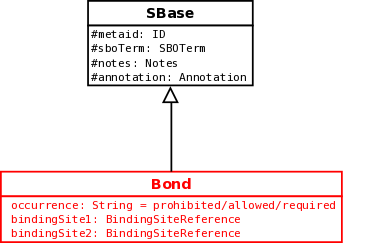
\includegraphics[scale=0.5]{figs/pngs/BondClass.png} 
\caption{Definition of \class{Bond} and its relation with \class{SBase}.}
\label{fig:BondClass}
\end{center}
\end{figure}

\begin{example}
<multi:bond xmlns:multi="http://www.sbml.org/sbml/level3/version1/multi/version1" 
            multi:occurrence="required" />
  <!-- some binding site references -->
</multi:bond>
\end{example}

\subsection{BindingSiteReference}

A component involved in a bond is specified by a \class{BindingSiteReference}. As all elements derived from \class{SBase}, it can link to \class{Notes} and \class{Annotation}, and carry a \attribute{metaid}, and an \attribute{sboTerm}. In addition, a \class{BindingSiteReference} refers to the component involved in the bond through the attribute \attribute{speciesTypeState}, that points to the value of the \attribute{id} attribute of the relevant \class{SpeciesTypeState}.

\begin{figure}[H]
\begin{center}
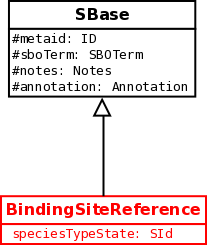
\includegraphics[scale=0.3]{figs/pngs/BindingSiteReferenceClass.png} 
\caption{Definition of \class{BindingSiteReference} and its relation with \class{SBase}.}
\label{fig:BindingSiteReferenceClass}
\end{center}
\end{figure}

\begin{example}
<multi:bindingSiteReference 
                    xmlns:multi="http://www.sbml.org/sbml/level3/version1/multi/version1" 
                    multi:speciesTypeState="speciesTypeState1" />
\end{example}

\subsection{Defining the components and the states allowed by the selector}

The following code contains a portion of selector describing two species type states, \cdata{speciesTypeState1} and \cdata{speciesTypeState2}. \cdata{SpeciesTypeState1} has a feature \cdata{stateFeature1} that can take the values \cdata{possibleValue1} or \cdata{possibleValue2} to pass the selection. In addition \cdata{speciesTypeState2} contains 4 instances of \cdata{speciesType2} (more exactly, it can contain between 4 and 4  instances of \cdata{speciesTypeState2} \ldots). The boolean attributes \attribute{connex} and \attribute{saturated} are of no use in this particular example, but are to be interpreted in conjunction with the bond definitions. 

\begin{example}
<multi:listOfSpeciesTypeStates
                  xmlns:multi="http://www.sbml.org/sbml/level3/version1/multi/version1">
  <multi:speciesTypeState multi:id="speciesTypeState1" multi:speciesType="speciesType1" 
                          multi:minOccur="4" multi:maxOccur="4" 
                          multi:connex="true" multi:saturated="true">
    <multi:listOfStateFeatureInstances>
      <multi:stateFeatureInstance multi:stateFeature="stateFeature1">
        <multi:listOfStateFeatureValues>
          <multi:stateFeatureValue multi:possibleValue="possibleValue1" />
          <multi:stateFeatureValue multi:possibleValue="possibleValue2" />
        </multi:listOfStateFeatureValues>
      </multi:stateFeatureInstance>
    </multi:listOfStateFeatureInstances>
  </multi:speciesTypeState>
  <multi:speciesTypeState multi:id="speciesTypeState2" multi:speciesType="speciesType2"
                          multi:minOccur="1" multi:maxOccur="1">
    <multi:listOfContainedSpeciesTypes>
      <multi:containedSpeciesType multi:speciesTypeState="speciesTypeState1" />
    </multi:listOfContainedSpeciesTypes>
  </multi:speciesTypeState>
</multi:listOfSpeciesTypeStates>
\end{example}

\begin{figure}[H]
\begin{center}
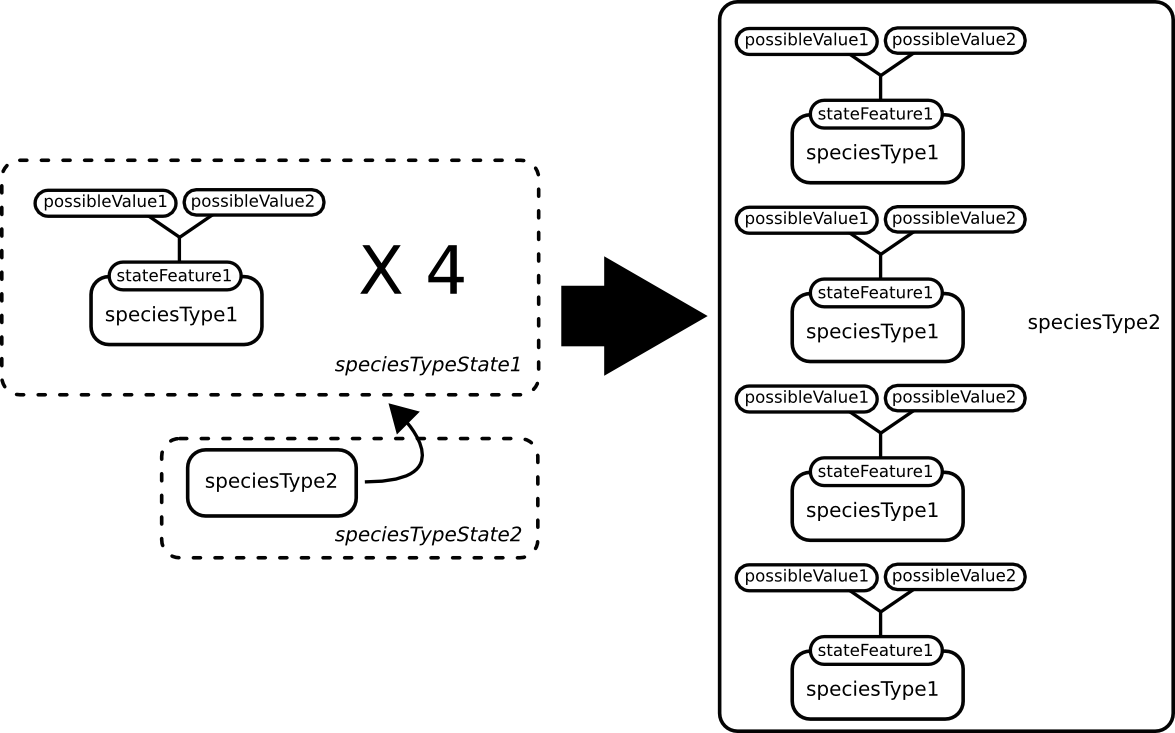
\includegraphics[scale=0.7]{figs/pngs/ex_sts.png} 
\caption{Generation of a nested selector from the definition of the two species type states, and the containment of one by the other.}
\label{fig:ex_sts}
\end{center}
\end{figure}

It is up to the model designer to avoid impossible structures, such as a species type state 1 that contains a species type 2, 2 itself containing 1. The following example is forbidden.

\color{red}
\begin{example}
<multi:listOfSpeciesTypeStates
                  xmlns:multi="http://www.sbml.org/sbml/level3/version1/multi/version1">
  <multi:speciesTypeState multi:id="speciesTypeState1" multi:speciesType="speciesType1" 
                          multi:minOccur="1" multi:maxOccur="1" >
    <multi:listOfContainedSpeciesTypes>
      <multi:containedSpeciesType multi:speciesTypeState="speciesTypeState2" />
    </multi:listOfContainedSpeciesTypes>
  </multi:speciesTypeState>
  <multi:speciesTypeState multi:id="speciesTypeState2" multi:speciesType="speciesType2"
                          multi:minOccur="1" multi:maxOccur="1" >
    <multi:listOfContainedSpeciesTypes>
      <multi:containedSpeciesType multi:speciesTypeState="speciesTypeState1" />
    </multi:listOfContainedSpeciesTypes>
  </multi:speciesTypeState>
</multi:listOfSpeciesTypeStates>
\end{example}
\normalcolor

If a species type is used in two different contexts, requiring for instance different numbers of occurrences,  two different species type states must be defined. For instance, if a species type A is used on its own in a species type C, or as contained twice in another species type B itself in C,  we need one A with min/maxOccur=1 and one A with min/maxOccur=2.

\begin{example}
<multi:listOfSpeciesTypeStates xmlns:multi="http://www.sbml.org/sbml/level3/version1/multi/version1">
  <multi:speciesTypeState multi:id="speciesTypeStateA1" multi:speciesType="speciesTypeA" 
                          multi:minOccur="1" multi:maxOccur="1" />
  <multi:speciesTypeState multi:id="speciesTypeStateA2" multi:speciesType="speciesTypeA"
                          multi:minOccur="2" multi:maxOccur="2" />
  <multi:speciesTypeState multi:id="speciesTypeStateB" multi:speciesType="speciesTypeB"
                          multi:minOccur="1" multi:maxOccur="1">
    <multi:listOfContainedSpeciesTypes>
      <multi:containedSpeciesType multi:speciesTypeState="speciesTypeStateA2" />
    </multi:listOfContainedSpeciesTypes>
  </multi:speciesTypeState>
  <multi:speciesTypeState multi:id="speciesTypeStateC" multi:speciesType="speciesTypeC"
                          multi:minOccur="1" multi:maxOccur="1" >
    <multi:listOfContainedSpeciesTypes>
      <multi:containedSpeciesType multi:speciesTypeState="speciesTypeStateA1" />
      <multi:containedSpeciesType multi:speciesTypeState="speciesTypeStateB" />
    </multi:listOfContainedSpeciesTypes>
  </multi:speciesTypeState>
</multi:listOfSpeciesTypeStates>
\end{example}

\begin{figure}[H]
\begin{center}
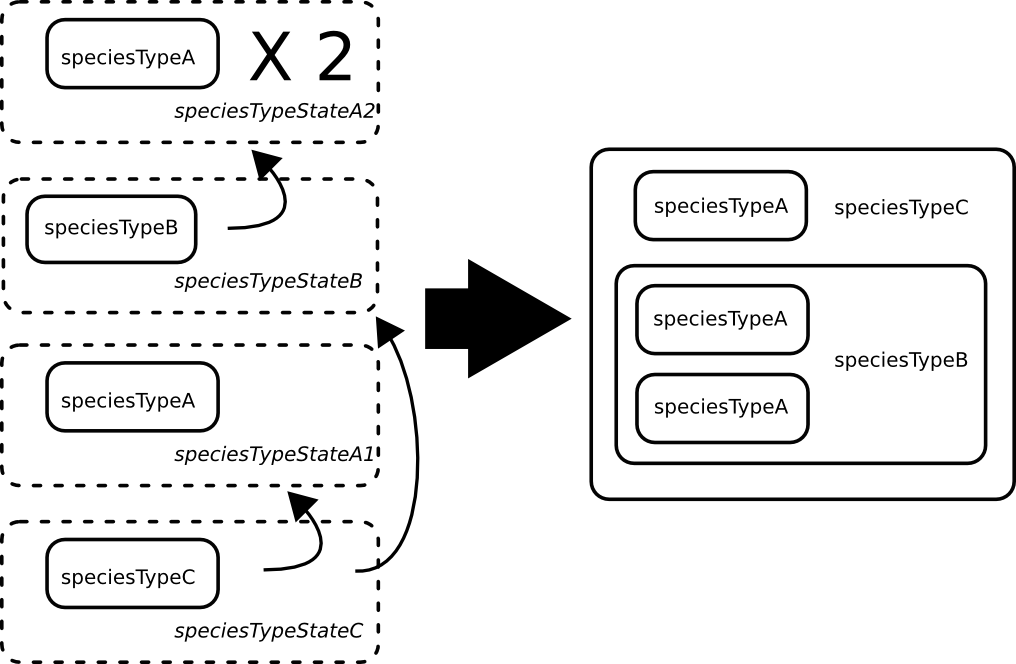
\includegraphics[scale=0.7]{figs/pngs/ex_sts_multiple.png} 
\caption{Nested selector where a given species type is used in two different contexts.}
\label{fig:ex_sts_multiple}
\end{center}
\end{figure}

The same species type can also be declared several time with different state feature values. The following example depicts a species type B containing two instances of species type A with a state feature displaying alternative values. Although in both case, the species type states refer to the same species type, we need to declare them separately.

\begin{example}
<multi:listOfSpeciesTypeStates
                   xmlns:multi="http://www.sbml.org/sbml/level3/version1/multi/version1">
  <multi:speciesTypeState multi:id="speciesTypeStateA1" multi:speciesType="speciesTypeA" 
                          multi:minOccur="1" multi:maxOccur="1" 
    <multi:listOfStateFeatureInstances>
      <multi:stateFeatureInstance multi:stateFeature="stateFeature1">
        <multi:listOfStateFeatureValues>
          <multi:stateFeatureValue multi:possibleValue="possibleValue1" />
        </multi:listOfStateFeatureValues>
      </multi:stateFeatureInstance>
    </multi:listOfStateFeatureInstances>
  </multi:speciesTypeState>
  <multi:speciesTypeState multi:id="speciesTypeStateA2" multi:speciesType="speciesTypeA" 
                          multi:minOccur="1" multi:maxOccur="1" 
    <multi:listOfStateFeatureInstances>
      <multi:stateFeatureInstance multi:stateFeature="stateFeature1">
        <multi:listOfStateFeatureValues>
          <multi:stateFeatureValue multi:possibleValue="possibleValue2" />
        </multi:listOfStateFeatureValues>
      </multi:stateFeatureInstance>
    </multi:listOfStateFeatureInstances>
  </multi:speciesTypeState>
  <multi:speciesTypeState multi:id="speciesTypeStateB" multi:speciesType="speciesTypeB"
                          multi:minOccur="1" multi:maxOccur="1">
    <multi:listOfContainedSpeciesTypes>
      <multi:containedSpeciesType multi:speciesTypeState="speciesTypeStateA1" />
      <multi:containedSpeciesType multi:speciesTypeState="speciesTypeStateA2" />
    </multi:listOfContainedSpeciesTypes>
  </multi:speciesTypeState>
</multi:listOfSpeciesTypeStates>
\end{example}

\begin{figure}[H]
\begin{center}
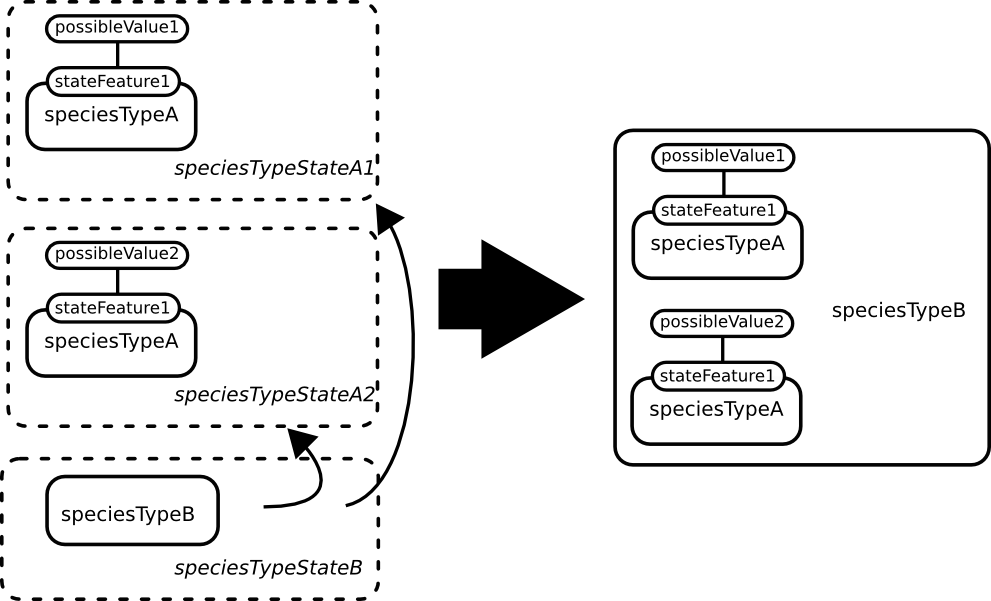
\includegraphics[scale=0.7]{figs/pngs/ex_sts_differentStates.png} 
\caption{Nested selector where a given species type is used with two different state feature values.}
\label{fig:ex_sts_differentStates}
\end{center}
\end{figure}

\subsection{Defining the connectivities allowed by the selector}
 
In a selector, instances of species types possessing an attribute \attribute{bindingSite} set to \cdata{true} can be referred to when they are involved in bonds, or explicitly listed as unbound. As a result such a species type can be used in four different contexts:

\begin{itemize}
 \item In a declared explicit bond, with another specific instance of a species type (represented by a bond linking two black entities in the example graphs). 

\begin{example}
<multi:bond xmlns:multi="http://www.sbml.org/sbml/level3/version1/multi/version1" 
            multi:occurrence="required" >
  <multi:bindingSiteReference multi:speciesTypeState="speciesTypeState1" />
  <multi:bindingSiteReference multi:speciesTypeState="speciesTypeState2" />
</multi:bond>
\end{example}

 \item In a declared generic bond without another specific instance of a species type (represented by an unlinked black entity in the example graphs). 

\begin{example}
<multi:bond xmlns:multi="http://www.sbml.org/sbml/level3/version1/multi/version1" 
            multi:occurrence="required" >
  <multi:bindingSiteReference multi:speciesTypeState="speciesTypeState1" />
</multi:bond>
\end{example}

 \item Declared as explicitly unbound (represented by a white entity in the example graphs). 

\begin{example}
<multi:listOfUnboundBindingSites 
             xmlns:multi="http://www.sbml.org/sbml/level3/version1/multi/version1" />
  <multi:bindingSiteReference multi:speciesTypeState="speciesTypeState1" />
</multi:listOfUnboundBindingSites>
\end{example}

\item Undeclared, meaning that one does not care if it is bound or not (represented by a gray entity in the example graphs). 
\end{itemize}

A given binding site can only be bound to another binding site. If three instances of species types are bound together, they have to be bound through different contained binding sites. Those binding sites can be different instances of the same species type (``identical'' binding sites) or instances of different species types (different binding sites). The following example is forbidden:

\color{red}
\begin{example}
<multi:listOfBonds xmlns:multi="http://www.sbml.org/sbml/level3/version1/multi/version1">
  <multi:bond multi:occurrence="required" >
    <multi:bindingSiteReference multi:speciesTypeState="speciesTypeStateA" />
    <multi:bindingSiteReference multi:speciesTypeState="speciesTypeStateB" />
  </multi:bond>
  <multi:bond multi:occurrence="required" >
    <multi:bindingSiteReference multi:speciesTypeState="speciesTypeStateA" />
    <multi:bindingSiteReference multi:speciesTypeState="speciesTypeStateC" />
  </multi:bond>
</multi:listOfBonds>
\end{example}
\normalcolor

Instead the following code should be used, where \cdata{speciesTypeStateA1} and \cdata{speciesTypeStateA2} are two different species type states of the same species type.

\color{blue}
\begin{example}
<multi:listOfBonds xmlns:multi="http://www.sbml.org/sbml/level3/version1/multi/version1">
  <multi:bond multi:occurrence="required" >
    <multi:bindingSiteReference multi:speciesTypeState="speciesTypeStateA1" />
    <multi:bindingSiteReference multi:speciesTypeState="speciesTypeStateB" />
  </multi:bond>
  <multi:bond multi:occurrence="required" >
    <multi:bindingSiteReference multi:speciesTypeState="speciesTypeStateA2" />
    <multi:bindingSiteReference multi:speciesTypeState="speciesTypeStateC" />
  </multi:bond>
</multi:listOfBonds>
\end{example}
\normalcolor

\begin{figure}[H]
\begin{center}
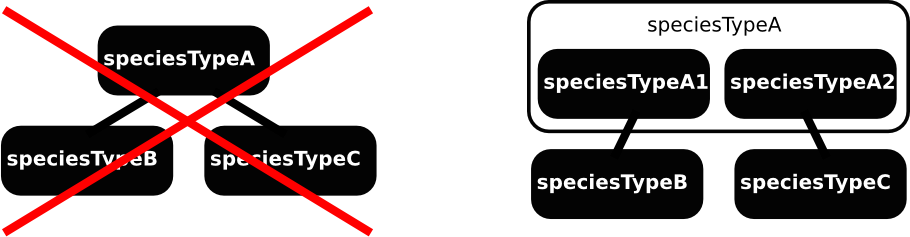
\includegraphics[scale=0.7]{figs/pngs/ex_multipleBinding.png} 
\caption{The connectivity on the left is forbidden, and the connectivity on the right should be used instead.}
\label{fig:ex_multipleBinding}
\end{center}
\end{figure}

The description of the connectivity through the list of bonds and the list of unbound binding sites is greedy. In other words, the possible connectivity is the sum of all the different listed possibilities. If in a selector, an instance of a species type is involved in at least one allowed bond, then it must be bound to something. It cannot be unbound. Furthermore, if an instance of a species type is involved in listed bonds, only the listed bonds can fulfill the selection. 

The attribute \attribute{occurrence}, in combination with explicit, generic and undeclared bonds, provides for a complete boolean logic to select the context of bindingSites. Note that \attribute{occurrence} is only present on \class{Bond}. In order to forbid a binding site to be unbound, we create a generic bond with \attribute{occurrence} set to \cdata{required} (to say that X cannot be free is equivalent to say that X had to be bound to something, whatever it is).

To exemplify this boolean logic, let's take the example of an instance of a species type X interacting with instances of species type A, B or C.

In the following code, X is not declared at all, therefore X can be bound to A, B, C or be unbound:

\begin{example}
<multi:selector xmlns:multi="http://www.sbml.org/sbml/level3/version1/multi/version1" 
                multi:id="selector1" />
  <multi:listOfSpeciesTypeStates>
    <multi:speciesTypeState id="speciesTypeStateA" speciesType="speciesTypeA"                                           
                            multi:minOccur="1" multi:maxOccur="1" />
    <multi:speciesTypeState id="speciesTypeStateB" speciesType="speciesTypeB"                           
                            multi:minOccur="1" multi:maxOccur="1" />
  </multi:listOfSpeciesTypeStates>
</multi:selector> 
\end{example}

With the following code, X can only be bound to A, or unbound:

\begin{example}
<multi:selector xmlns:multi="http://www.sbml.org/sbml/level3/version1/multi/version1" 
                multi:id="selector1" />
  <multi:listOfSpeciesTypeStates>
    <multi:speciesTypeState id="speciesTypeStateX" speciesType="speciesTypeX"                                           
                            multi:minOccur="1" multi:maxOccur="1" />
    <multi:speciesTypeState id="speciesTypeStateA" speciesType="speciesTypeA"                           
                            multi:minOccur="1" multi:maxOccur="1" />
  </multi:listOfSpeciesTypeStates>
  <multi:listOfBonds xmlns:multi="http://www.sbml.org/sbml/level3/version1/multi/version1" >
    <multi:bond multi:occurrence="allowed" >
      <multi:bindingSiteReference multi:speciesTypeState="speciesTypeStateX" />
      <multi:bindingSiteReference multi:speciesTypeState="speciesTypeStateA" />
    </multi:bond>
  </multi:listOfBonds>
</multi:selector> 
\end{example}

With the following code X can only be bound either to A or B, but not C:

\begin{example}
<multi:selector xmlns:multi="http://www.sbml.org/sbml/level3/version1/multi/version1" 
                multi:id="selector1" />
  <multi:listOfSpeciesTypeStates>
    <multi:speciesTypeState id="speciesTypeStateX" speciesType="speciesTypeX"                                           
                            multi:minOccur="1" multi:maxOccur="1" />
    <multi:speciesTypeState id="speciesTypeStateA" speciesType="speciesTypeA"                           
                            multi:minOccur="1" multi:maxOccur="1" />
    <multi:speciesTypeState id="speciesTypeStateB" speciesType="speciesTypeB"                           
                            multi:minOccur="1" multi:maxOccur="1" />
  </multi:listOfSpeciesTypeStates>
  <multi:listOfBonds xmlns:multi="http://www.sbml.org/sbml/level3/version1/multi/version1">
    <multi:bond multi:occurrence="allowed" >
      <multi:bindingSiteReference multi:speciesTypeState="speciesTypeStateX" />
      <multi:bindingSiteReference multi:speciesTypeState="speciesTypeStateA" />
    </multi:bond>
    <multi:bond multi:occurrence="allowed" >
      <multi:bindingSiteReference multi:speciesTypeState="speciesTypeStateX" />
      <multi:bindingSiteReference multi:speciesTypeState="speciesTypeStateB" />
    </multi:bond>
  </multi:listOfBonds>
</multi:selector> 
\end{example}

The following code defines a generic bond with X, which mean that X can be bound to A, B or C, but has to be bound to something:

\begin{example}
<multi:selector xmlns:multi="http://www.sbml.org/sbml/level3/version1/multi/version1" 
                multi:id="selector1" />
  <multi:listOfSpeciesTypeStates>
    <multi:speciesTypeState id="speciesTypeStateX" speciesType="speciesTypeX"                                           
                            multi:minOccur="1" multi:maxOccur="1" />
  </multi:listOfSpeciesTypeStates>
  <multi:listOfBonds xmlns:multi="http://www.sbml.org/sbml/level3/version1/multi/version1" >
    <multi:bond multi:occurrence="allowed" >
      <multi:bindingSiteReference multi:speciesTypeState="speciesTypeStateX" />
    </multi:bond>
  </multi:listOfBonds>
</multi:selector> 
\end{example}

The following code says that X cannot be bound to C (The bond X-C is prohibited), and therefore has to be bound to A or B or unbound.

\begin{example}
<multi:selector xmlns:multi="http://www.sbml.org/sbml/level3/version1/multi/version1" 
                multi:id="selector1" />
  <multi:listOfSpeciesTypeStates>
    <multi:speciesTypeState id="speciesTypeStateX" speciesType="speciesTypeX"                                           
                            multi:minOccur="1" multi:maxOccur="1" />
    <multi:speciesTypeState id="speciesTypeStateC" speciesType="speciesTypeC"                           
                            multi:minOccur="1" multi:maxOccur="1" />
  </multi:listOfSpeciesTypeStates>
  <multi:listOfBonds xmlns:multi="http://www.sbml.org/sbml/level3/version1/multi/version1">
    <multi:bond multi:occurrence="prohibited" >
      <multi:bindingSiteReference multi:speciesTypeState="speciesTypeStateX" />
      <multi:bindingSiteReference multi:speciesTypeState="speciesTypeStateC" />
    </multi:bond>
  </multi:listOfBonds>
</multi:selector> 
\end{example}
 
The following code says that X cannot be bound to C (The bond X-C is prohibited), however a generic bond specifies that X has to bound to something, therefore effectively to A or B. In this particular example, \attribute{occurrence} on the generic bond can be set indifferently to \cdata{allowed} or \cdata{required}.

\begin{example}
<multi:selector xmlns:multi="http://www.sbml.org/sbml/level3/version1/multi/version1" 
                multi:id="selector1" />
  <multi:listOfSpeciesTypeStates>
    <multi:speciesTypeState id="speciesTypeStateX" speciesType="speciesTypeX"                                           
                            multi:minOccur="1" multi:maxOccur="1" />
    <multi:speciesTypeState id="speciesTypeStateC" speciesType="speciesTypeC"                           
                            multi:minOccur="1" multi:maxOccur="1" />
  </multi:listOfSpeciesTypeStates>
  <multi:listOfBonds xmlns:multi="http://www.sbml.org/sbml/level3/version1/multi/version1" >
    <multi:bond multi:occurrence="prohibited" >
      <multi:bindingSiteReference multi:speciesTypeState="speciesTypeStateX" />
      <multi:bindingSiteReference multi:speciesTypeState="speciesTypeStateC" />
    </multi:bond>
    <multi:bond multi:occurrence="allowed" >
      <multi:bindingSiteReference multi:speciesTypeState="speciesTypeStateX" />
    </multi:bond>
  </multi:listOfBonds>
</multi:selector> 
\end{example}

The following case is overdetermined, since the impossibility for X to bind C is implicit in the restriction of its binding to A or B.

\begin{example}
<multi:selector xmlns:multi="http://www.sbml.org/sbml/level3/version1/multi/version1" 
                multi:id="selector1" />
  <multi:listOfSpeciesTypeStates>
    <multi:speciesTypeState id="speciesTypeStateX" speciesType="speciesTypeX"                                           
                            multi:minOccur="1" multi:maxOccur="1" />
    <multi:speciesTypeState id="speciesTypeStateA" speciesType="speciesTypeA"                           
                            multi:minOccur="1" multi:maxOccur="1" />
    <multi:speciesTypeState id="speciesTypeStateB" speciesType="speciesTypeB"                           
                            multi:minOccur="1" multi:maxOccur="1" />
    <multi:speciesTypeState id="speciesTypeStateC" speciesType="speciesTypeC"                           
                            multi:minOccur="1" multi:maxOccur="1" />
  </multi:listOfSpeciesTypeStates>
  <multi:listOfBonds xmlns:multi="http://www.sbml.org/sbml/level3/version1/multi/version1">
    <multi:bond multi:occurrence="allowed" >
      <multi:bindingSiteReference multi:speciesTypeState="speciesTypeStateX" />
      <multi:bindingSiteReference multi:speciesTypeState="speciesTypeStateA" />
    </multi:bond>
    <multi:bond multi:occurrence="allowed" >
      <multi:bindingSiteReference multi:speciesTypeState="speciesTypeStateX" />
      <multi:bindingSiteReference multi:speciesTypeState="speciesTypeStateB" />
    </multi:bond>
    <multi:bond multi:occurrence="prohibited" >
      <multi:bindingSiteReference multi:speciesTypeState="speciesTypeStateX" />
      <multi:bindingSiteReference multi:speciesTypeState="speciesTypeStateC" />
    </multi:bond>
  </multi:listOfBonds>
</multi:selector> 
\end{example}

The boolean attributes \attribute{connex} and \attribute{saturated} precise the topology of a multimeric assembly of the same component (same species type state, that is same species type with the same values allowed for all their state features). One can then declare the component only once, and each of the bond types or unbound binding sites only once. Attribute \attribute{saturated} set to \cdata{true} means that all the contained species types which \attribute{bindingSite} is set to \cdata{true} have to be bound. Attribute \attribute{connex} means that all the instances of the species type state have to be connected within the same complex. The following example presents a tetramer of identical subunits. 

\begin{example}
<multi:selector xmlns:multi="http://www.sbml.org/sbml/level3/version1/multi/version1" 
                multi:id="selector1" />
  <multi:listOfSpeciesTypeStates>
    <multi:speciesTypeState id="speciesTypeStateA" speciesType="speciesTypeA"                                           
                            multi:minOccur="4" multi:maxOccur="4"
                            connex="{true|false}" saturated="{true|false}">
      <multi:listOfContainedSpeciesTypes>
        <multi:containedSpeciesType multi:speciesTypeState="speciesTypeStateB" />
        <multi:containedSpeciesType multi:speciesTypeState="speciesTypeStateC" />
      </multi:listOfContainedSpeciesTypes>
    </multi:speciesTypeState>
    <multi:speciesTypeState id="speciesTypeStateB" speciesType="speciesTypeB"                                           
                            multi:minOccur="1" multi:maxOccur="1" />
    <multi:speciesTypeState id="speciesTypeStateC" speciesType="speciesTypeC"                                           
                            multi:minOccur="1" multi:maxOccur="1" />
  </multi:listOfSpeciesTypeStates>
  <multi:listOfBonds xmlns:multi="http://www.sbml.org/sbml/level3/version1/multi/version1">
    <multi:bond multi:occurrence="allowed" >
      <multi:bindingSiteReference multi:speciesTypeState="speciesTypeStateB" />
      <multi:bindingSiteReference multi:speciesTypeState="speciesTypeStateC" />
    </multi:bond>
  </multi:listOfBonds>
</multi:selector> 
\end{example}

The following graphs are examples of the various combinations possible of \attribute{connex} and \attribute{saturated} attributes. 

\begin{figure}[H]
\begin{center}
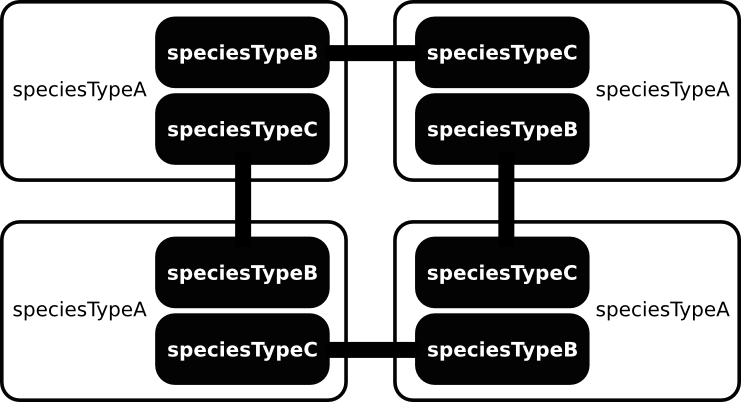
\includegraphics[scale=0.7]{figs/pngs/ex_connex-saturated.png} 
\caption{\xmlcode{connex="true" saturated="true"}}
\label{fig:ex_connex-saturated}
\end{center}
\end{figure}

\begin{figure}[H]
\begin{center}
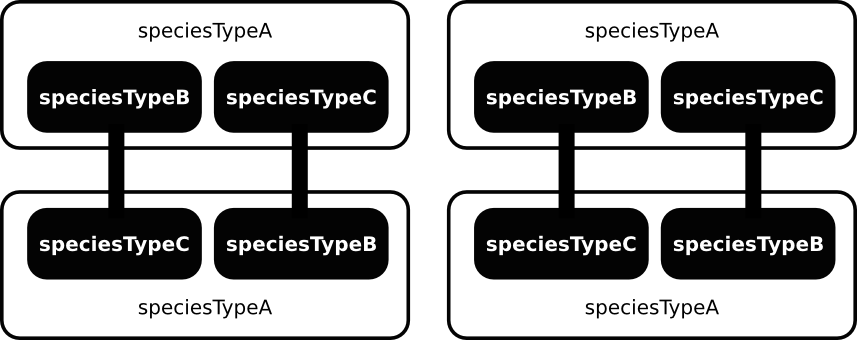
\includegraphics[scale=0.7]{figs/pngs/ex_nonconnex-saturated.png} 
\caption{\xmlcode{connex="false" saturated="true"}}
\label{fig:ex_nonconnex-saturated}
\end{center}
\end{figure}

\begin{figure}[H]
\begin{center}
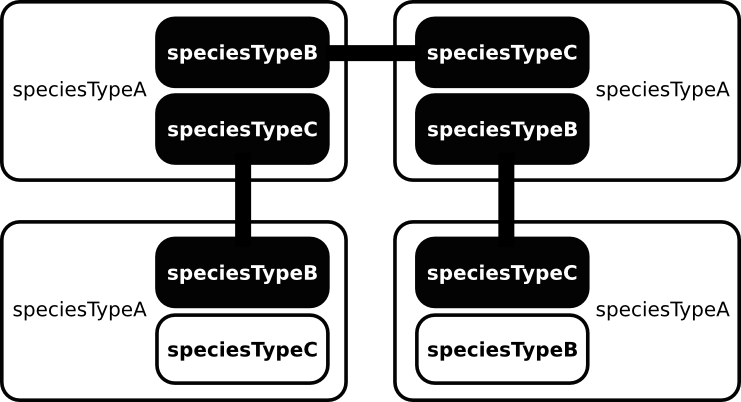
\includegraphics[scale=0.7]{figs/pngs/ex_connex-nonsaturated.png} 
\caption{\xmlcode{connex="true" saturated="false"}}
\label{fig:ex_connex-nonsaturated}
\end{center}
\end{figure}

\begin{figure}[H]
\begin{center}
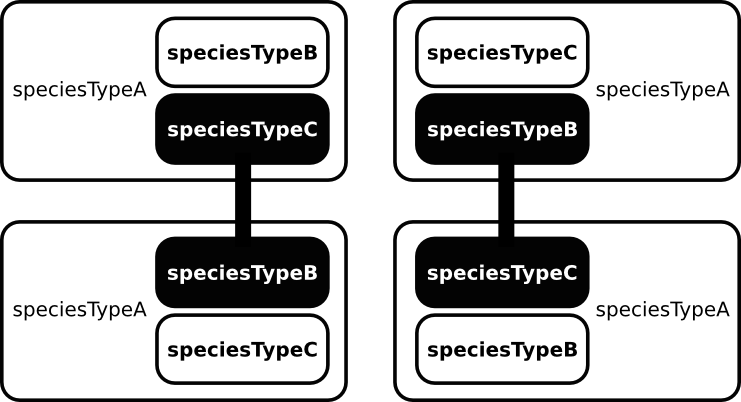
\includegraphics[scale=0.7]{figs/pngs/ex_nonconnex-nonsaturated.png} 
\caption{\xmlcode{connex="false" saturated="false"}}
\label{fig:ex_nonconnex-nonsaturated}
\end{center}
\end{figure}

\section{Definition of the instances and pools of instances}

Once the multistate and multi-component types of entities used by the model have been described, using \class{SpeciesType}s and \class{Selector}s, one needs to define quantitatively actual states and connectivity of the elementary components within the \class{Species} of the SBML core. The new entity pool instances will then be used either as initial conditions or in any SBML constructs refering to \class{Species}. In order to specify these states and partnerships, we extend \class{Species} to link to \class{SpeciesTypeInstance}s, themselves refering to a list of \class{Selector}s. A \class{SpeciesTypeInstance} describes an entity that fulfils all the listed \class{Selector}s. A \class{Species} is effectively the ensemble of all the \class{SpeciesTypeInstance}s belonging to the same compartment. Note that it is the responsibility of the person or software generating the SBML file to ensure that the selectors used to precise the \class{SpeciesTypeInstance}s are not incompatible. The initial conditions, that is the intial states and connectivities of each species have to be fully specified.

\begin{figure}[h!]
\begin{center}
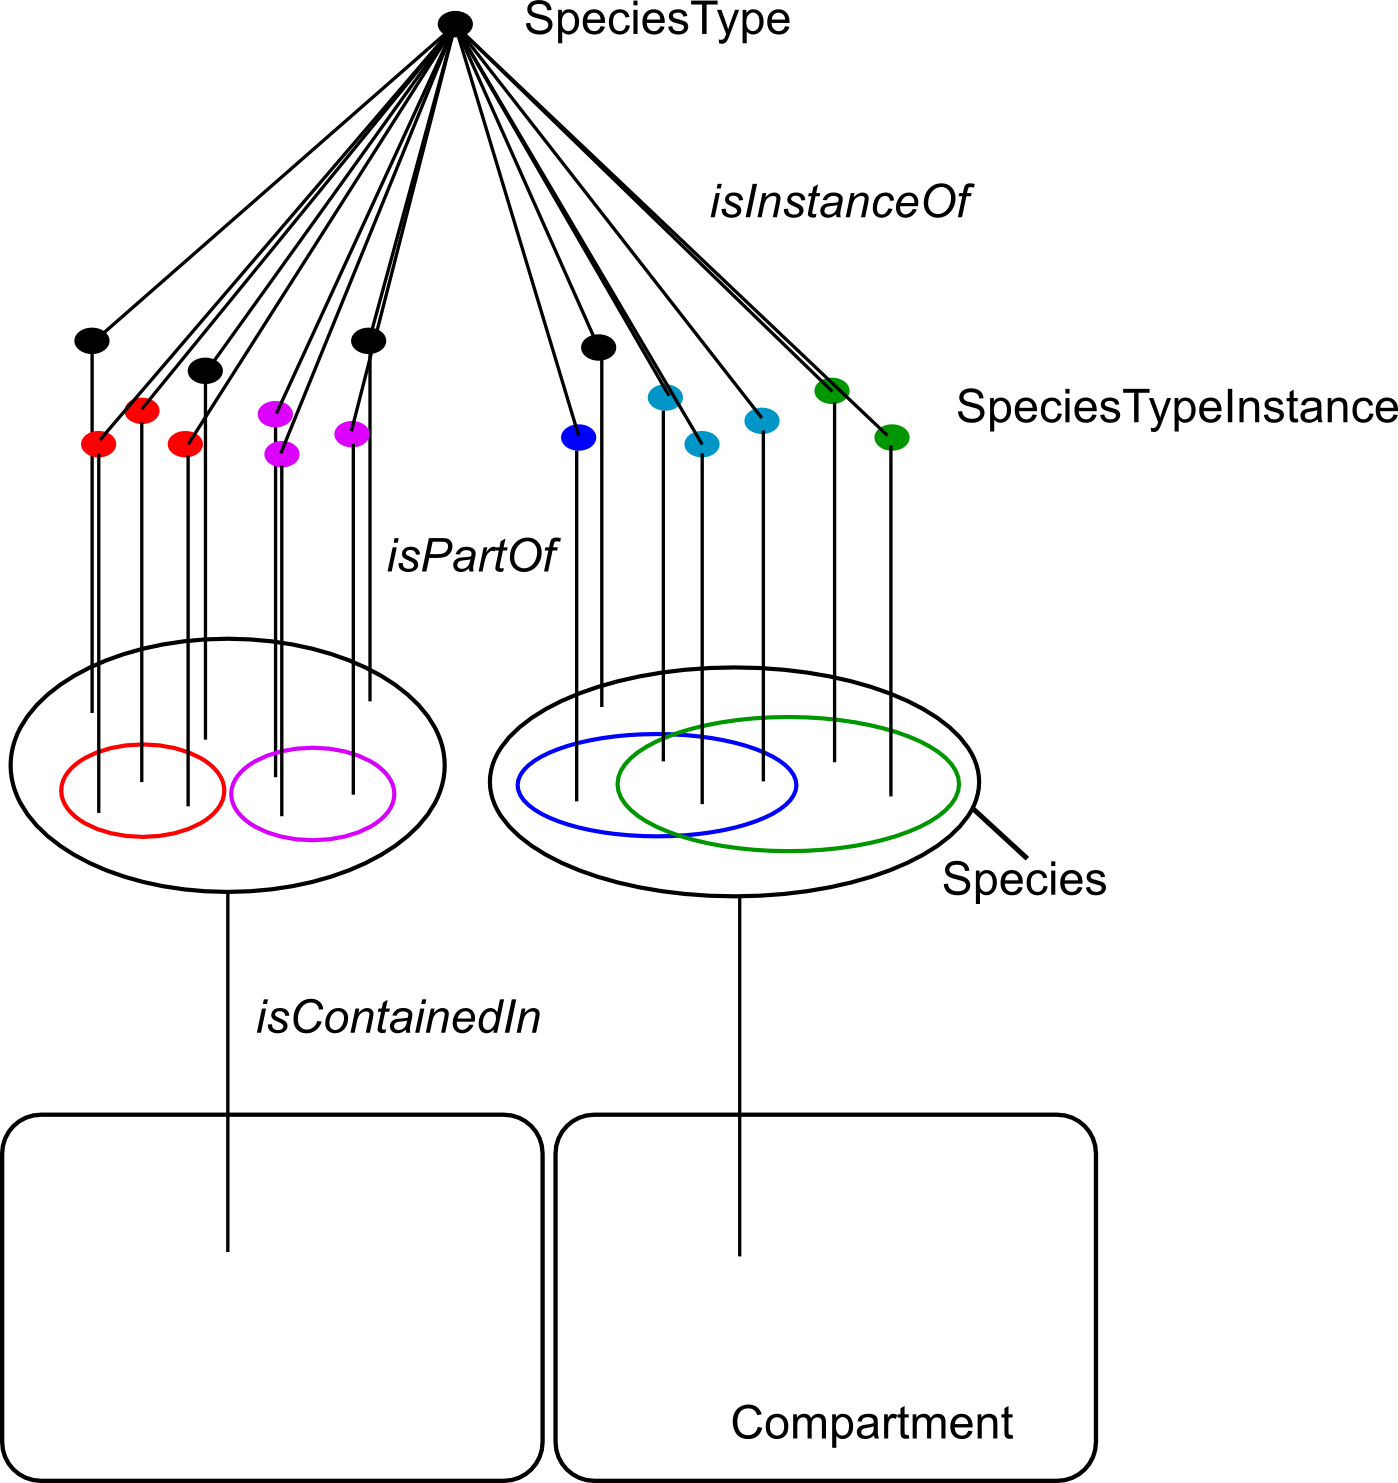
\includegraphics[scale=0.5]{./figs/pngs/Instantiation.png}
\caption{Relationships between a conceptual species type, the actual species type instances and the different pools of entities defined in a model description.}
\end{center}
\end{figure}

\begin{figure}[h!]
\begin{center}
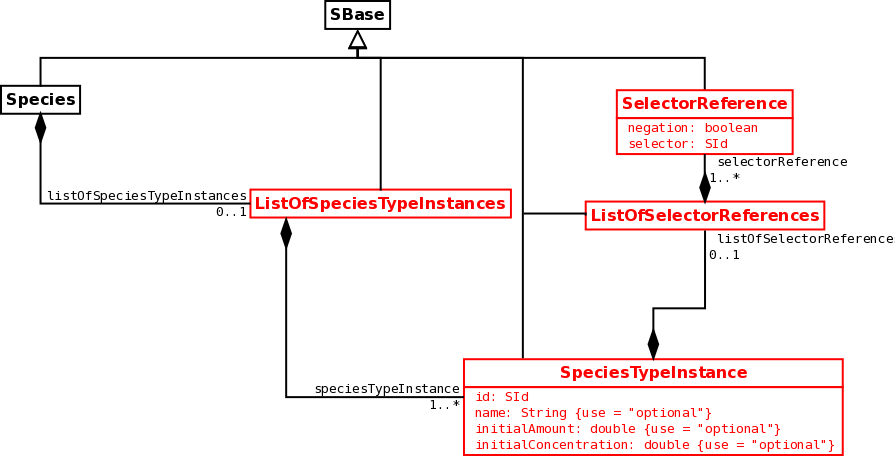
\includegraphics[scale=0.3]{./figs/pngs/SpeciesGeneral.png}
\caption{\class{Species} and all the associated classes of \multiVone.}
\end{center}
\end{figure}

Note that a ``filtered'' species is also an entity pool, and therefore is located in a given compartment. However, this species subset can be generated, selected, with a \class{Selector} that is using several SpeciesTypes instantiated by species in different compartments. Another species, located in another compartment, could be selected by a different "portion" of the same selector. This provides a mechanism to build multi-compartment entities.

\subsection{Species}

In order to encode the structures needed to refine entity pools based on their state and connectivity, we precise instances of which \class{SpeciesType} compose the \class{Species}. The element \class{Species} is then linked to a list of \class{SpeciesTypeInstance}s, each of one describing an entity part of a different pool.

\begin{figure}[H]
\begin{center}
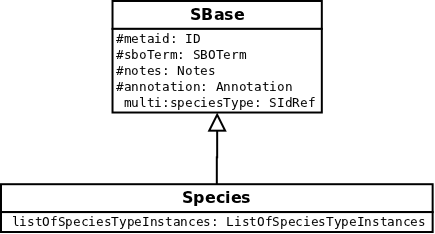
\includegraphics[scale=0.3]{figs/pngs/SpeciesClass.png} 
\caption{Definition of the extended version of \class{Species} and its relation with \class{SBase}.}
\label{fig:SpeciesClass}
\end{center}
\end{figure}

\begin{example}
<species id="species1" name="LGIC" sboTerm="SBO:0000245"
         boundaryCondition="false" hasOnlySubstanceUnit="false" constant="false"
         xmlns:multi="http://www.sbml.org/sbml/level3/version1/multi/version1"
         multi:speciesType="speciesType1" >
  <multi:listOfSpeciesTypeInstances>
    <!-- some definition of subpools -->
  </multi:listOfSpeciesTypeInstances>
</species>
\end{example}

\subsection{SpeciesTypeInstance}

A \class{SpeciesTypeInstance} is identified by an \attribute{id} and an optional \attribute{name}.  A \class{SpeciesTypeInstance} is linked to a list of \class{SelectorReference}s. When used in the SBML model, the \attribute{id} represent the either the size of the pool formed by all the \class{SpeciesTypeInstance}s that fulfil the selection, or the species type restriction. The context decides. As all elements derived from \class{SBase}, it can link to \class{Notes} and \class{Annotation}, and carry a \attribute{metaid}, and an \attribute{sboTerm}. In addition, a \class{SpeciesTypeInstance} may precise the size of the pool as an \attribute{initialAmount} or an \attribute{initialConcentration}. If neither \attribute{initialAmount} nor \attribute{initialConcentration} are precised, the instance is not to be used for initial conditions.  

\begin{figure}[H]
\begin{center}
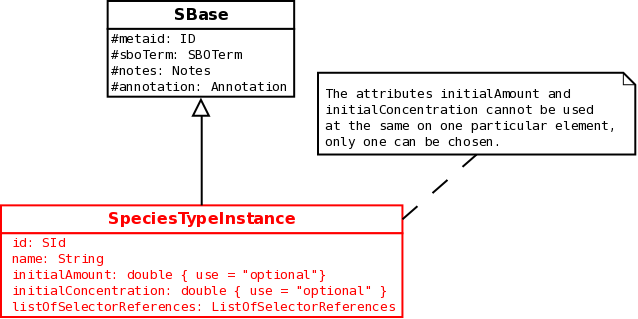
\includegraphics[scale=0.3]{figs/pngs/SpeciesTypeInstanceClass.png} 
\caption{Definition of \class{SpeciesTypeInstance} and its relation with \class{SBase}.}
\label{fig:SpeciesTypeInstanceClass}
\end{center}
\end{figure}

\begin{example}
<multi:speciesTypeInstance 
         xmlns:multi="http://www.sbml.org/sbml/level3/version1/multi/version1" 
         multi:id="SpeciesTypeInstance1"
         multi:name="LGIC_open"
         multi:initialAmount="1">
  <multi:listOfSelectorReferences>
    <!-- selectors to combine to filter out the instance -->
  </multi:listOfSelectorReferences>
</multi:speciesTypeInstance>
\end{example}

Note that because an instance can fulfill several selectors, the selectors used to create instances used as initial conditions may overlap. As a consequence, the sum of all the initial quantities may be larger than the initial quantity specified on the \class{Species}. It is up to the modeler generating the description to make sure there is no ambiguity and that whatever procedure is used to create the instances result in the same distribution.

\class{SpeciesTypeInstance}s defined in a \class{Species} inherit the value of the attribute \attribute{hasOnlySubstanceUnit} carried by the \class{Species}. In other words, regardless of the presence of the attributes \attribute{initialAmount} and \attribute{initialConcentration} carried by a \class{SpeciesTypeInstance}, when used in a context requiring a quantity its \attribute{id} represents an amount if  the \class{species}' \attribute{hasOnlySubstanceUnit} is set to \cdata{true}. 

\subsection{SelectorReference}\label{sec:SelectorReference}

As all elements derived from \class{SBase}, A \class{SelectorReference}  can link to \class{Notes} and \class{Annotation}, and carry a \attribute{metaid}, and an \attribute{sboTerm}. It targets a \class{Selector} through its \attribute{selector} attribute. A boolean attribute \attribute{negation} allows to precise that the entities fulfilling the rules described in the selector are NOT selected.

\begin{figure}[H]
\begin{center}
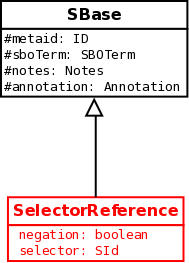
\includegraphics[scale=0.3]{figs/pngs/SelectorReferenceClass.png} 
\caption{Definition of \class{SelectorReference} and its relation with \class{SBase}.}
\label{fig:SelectorReferenceClass}
\end{center}
\end{figure}

\begin{example}
<multi:selectorReference 
         xmlns:multi="http://www.sbml.org/sbml/level3/version1/multi/version1" 
         multi:selector="selector1"
         multi:negation="true" />
\end{example}

\subsection{Complete description of a species with pools of instances}\label{exampleSpecies}

The example below describes the encoding of two instances of the speciesType \cdata{speciesType1}. 

\begin{example}
<species id="species1" 
         boundaryCondition=false" hasOnlySubstanceUnit=false" constant=false"
         compartment="compartment1" initialAmount="1000"
         xmlns:multi="http://www.sbml.org/sbml/level3/version1/multi/version1"
         multi:speciesType="speciesType1" >
  <multi:listOfSpeciesTypeInstances>
    <multi:SpeciesTypeInstance multi:id="speciesTypeInstance1" 
                               multi:initialAmount="1">
      <multi:listOfSelectorReferences>
        <multi:selectorReference multi:selector="selector1" multi:negation="false"/>
      <multi:listOfSelectorReferences>
    </multi:speciesTypeInstance>
    <multi:speciesTypeInstance multi:id="speciesTypeInstance2">
      <multi:listOfSelectorReferences>
        <multi:selectorReference multi:selector="selector2" multi:negation="false"/>
        <multi:selectorReference multi:selector="selector3" multi:negation="true" />
      <multi:listOfSelectorReferences>
    </multi:speciesTypeInstance>
  </multi:listOfSpeciesTypeInstances>
</species>
\end{example}

\begin{figure}[H]
\begin{center}
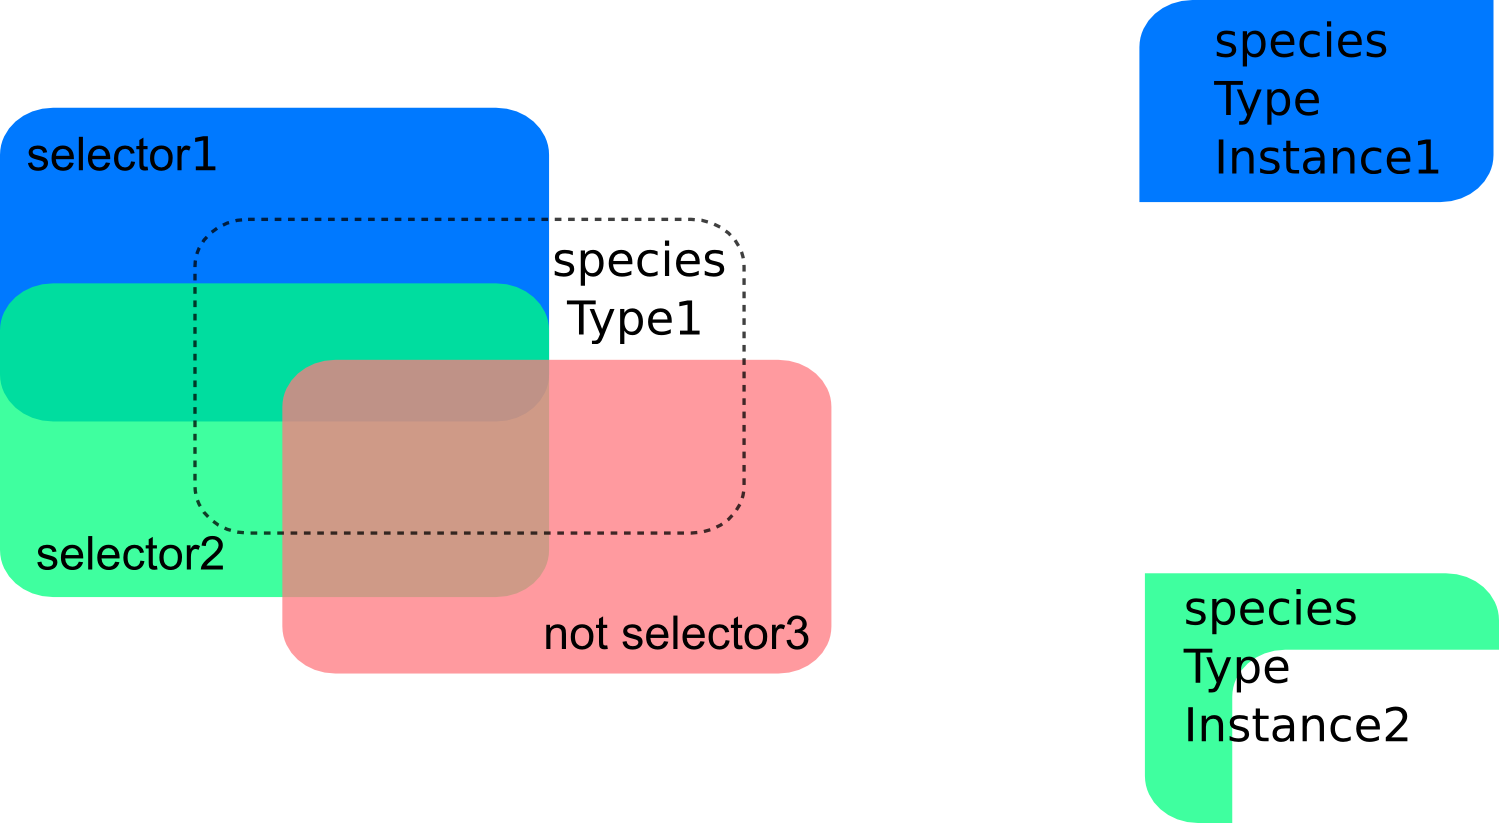
\includegraphics[scale=0.4]{figs/pngs/speciesTypeInstanceBuilding.png}
\caption{Procedure to build speciesTypeInstances from a speciesType and selectors. The dashed rectangle represent all the instances of a species, in all possible states and connectivity. Selector1 is used to generate the entity pool SpeciesTypeInstance1. Selector2 and Selector3 are used in combination to generate SpeciesTypeInstance2.}
\label{fig:speciesTypeInstanceBuilding}
\end{center}
\end{figure}



\section{Computing initial values for pools of instances}

In \sbmlLthreeVone, \class{InitialAssignment}s are used to assign initial values to variables of a model, that are \class{Compartment}s, \class{Species}, \class{SpeciesReference}, or global \class{Parameter}s.  In order to assign the value of a specific type of species, \class{InitialAssignment}s in \multiVone also contain an element \class{SpeciesTypeInstanceChange}. The assignment sets the initial quantity of instances that fulfil a certain selection using the mathematical expression provided. The value provided by the \class{InitialAssignment} overides the value provided by the attributes \attribute{initialAmount} or \attribute{initialConcentration} of the relevant \class{SpeciesTypeInstance}.

\begin{figure}[h!]
\begin{center}
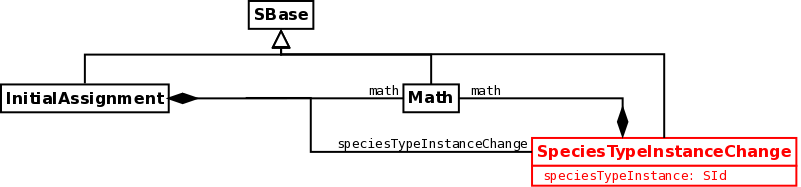
\includegraphics[scale=0.3]{./figs/pngs/InitialAssignmentGeneral.png}
\caption{\class{InitialAssignment} and all the associated classes of \multiVone.}
\end{center}
\end{figure}


\subsection{InitialAssignment}

In order to assign the initial values to entity subpools, defined by specific state and connectivity, the element \class{InitialAssignment} of \sbmlLthreeVone core is linked to a \class{SpeciesTypeInstanceChange}.

\begin{figure}[H]
\begin{center}
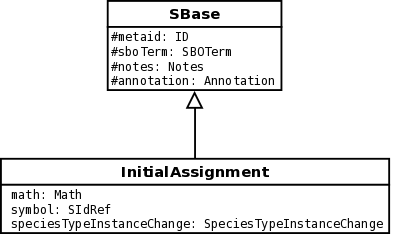
\includegraphics[scale=0.4]{figs/pngs/InitialAssignmentClass.png} 
\caption{Definition of the extended version of \class{InitialAssignment} and its relation with \class{SBase}.}
\label{fig:InitialAssignmentClass}
\end{center}
\end{figure}

\subsection{SpeciesTypeInstanceChange}\label{SpeciesTypeInstanceChange}

As all elements derived from \class{SBase}, A \class{SpeciesTypeInstanceChange} can link to \class{Notes} and \class{Annotation}, and carry a \attribute{metaid}, and an \attribute{sboTerm}. It targets a \class{SpeciesTypeInstance} through its \attribute{SpeciesTypeInstance} attribute. The change is computed using a MathML construct, as is always the case in \sbmlLthreeVone.

\begin{figure}[H]
\begin{center}
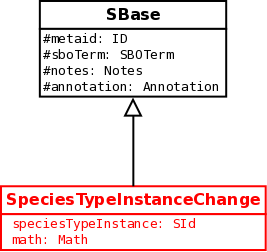
\includegraphics[scale=0.3]{figs/pngs/SpeciesTypeInstanceChangeClass.png} 
\caption{Definition of \class{SpeciesTypeInstanceChange} and its relation with \class{SBase}.}
\label{fig:SpeciesTypeInstanceChangeClass}
\end{center}
\end{figure}

\subsection{Complete example of an initial assignment}

The following example presents the assignment of the initial value for the subpool of \cdata{species1} defined as \cdata{speciesTypeInstance1}. This value is computed as the product of the parameters \cdata{x} and \cdata{y}, defined elsewhere. Note the empty \class{Math}, used when the software is unable to use the package \multiVone.

\begin{example}
<species id="species1" 
         boundaryCondition="false" hasOnlySubstanceUnit="false" constant="false"
         compartment="compartment1" initialAmount="1000"
         xmlns:multi="http://www.sbml.org/sbml/level3/version1/multi/version1"
         multi:speciesType="speciesType1" >
  <multi:listOfSpeciesTypeInstances>
    <multi:speciesTypeInstance multi:id="speciesTypeInstance1" multi:initialAmount="1">
      <multi:listOfSelectorReferences>
        <multi:selectorReference multi:selector="selector1" />
      <multi:listOfSelectorReferences>
    </multi:speciesTypeInstance>
  </multi:listOfSpeciesTypeInstances>
</species>
<initialAssignment symbol="species1">
  <multi:speciesTypeInstanceChange speciesTypeInstance="speciesTypeInstance1">
    <math xmlns="http://www.w3.org/1998/Math/MathML">
      <apply>
        <times/>
        <ci> x </ci>
        <ci> y </ci>
      </apply>
    </math>
  </multi:speciesTypeInstanceChange>
  <math xmlns="http://www.w3.org/1998/Math/MathML" />
</initialAssignment>
\end{example}
\section{Rules}

In \sbmlLthreeVone, \class{AssignmentRule}s and \class{RateRule}s are used to assign values or change of values respectively to variables of a model, that are \class{Compartment}s, \class{Species}, \class{SpeciesReference}, or global \class{Parameter}s.  In order to assign the value of a specific type of species, \class{AssignmentRule}s and  \class{RateRule}s in \multiVone also contain an element \class{SpeciesTypeInstanceChange}. The assignment sets the quantity of instances that fulfil a certain selection using the mathematical expression provided. 

\begin{figure}[h!]
\begin{center}
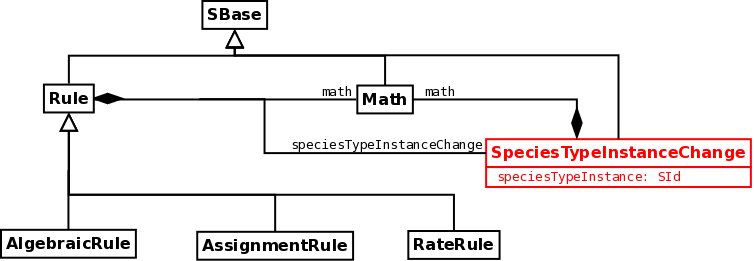
\includegraphics[scale=0.3]{./figs/pngs/RuleGeneral.png}
\caption{\class{Rule} and all the associated classes of \multiVone.}
\end{center}
\end{figure}

\subsection{Rule}

In order to assign values, or value evolutions, to entity subpools, defined by specific state and connectivity, the elements \class{AssignmentRule} and \class{RateRule} of \sbmlLthreeVone core are linked to a \class{SpeciesTypeInstanceChange}.

\begin{figure}[H]
\begin{center}
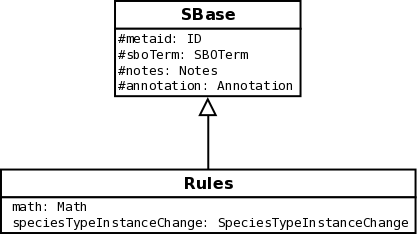
\includegraphics[scale=0.4]{figs/pngs/RuleClass.png} 
\caption{Definition of the extended version of \class{Rule} and its relation with \class{SBase}.}
\label{fig:RuleClass}
\end{center}
\end{figure}

\subsection{SpeciesTypeInstanceChange}

For a definition of \class{SpeciesTypeInstanceChange}, see section \ref{SpeciesTypeInstanceChange}.
\section{Definition of reactions and reaction rules}

Now that different instances of the species types have been defined using species and selectors, we can use them to choose between alternative conditional reactions, and to set-up the characteristics of the entities resulting from those conditional reactions. This is done by creating, for each relevant reaction, a list of reaction rules that contains alternative kineticLaws. 

\begin{figure}[h!]
\begin{center}
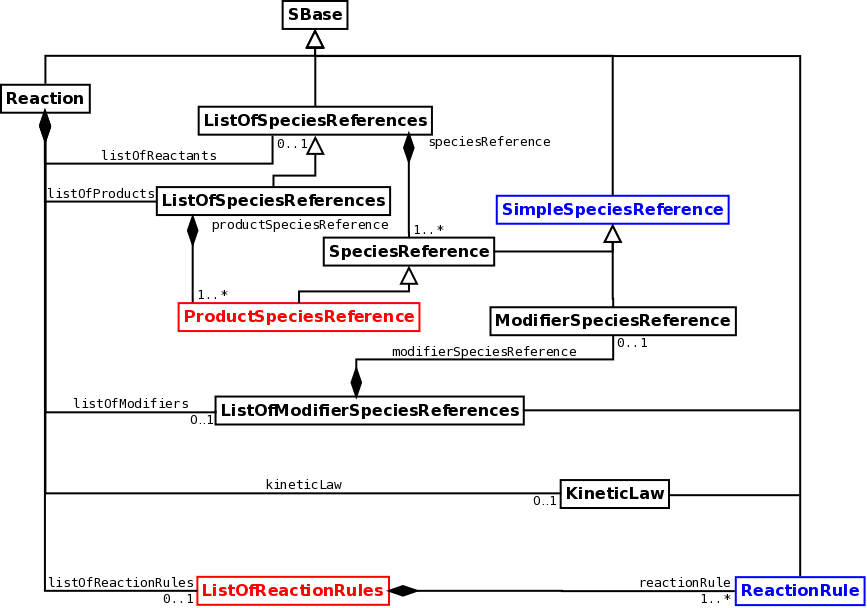
\includegraphics[scale=0.3]{./figs/pngs/ReactionGeneral.png}
\caption{\class{Reaction} and all the associated classes of \multiVone.}
\end{center}
\end{figure}

\begin{figure}[h!]
\begin{center}
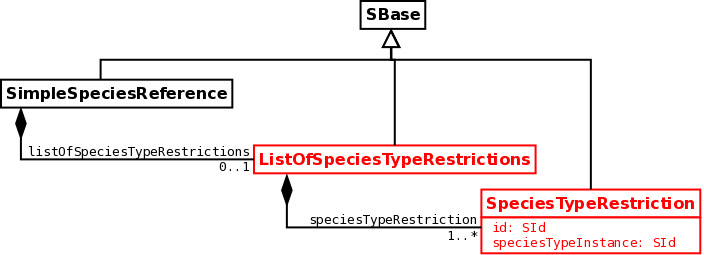
\includegraphics[scale=0.3]{./figs/pngs/SimpleSpeciesReferenceGeneral.png}
\caption{\class{SimpleSpeciesReference} and all the associated classes of \multiVone.}
\end{center}
\end{figure}

A reaction rule applies when a list of conditions is fulfiled by the reacting species, and a reaction rule produces outcomes described in a list of results. Reaction rules must not produce mass or cause unexplained disappearance of it. In other words, once the various selections are applied, what is on the left should be on the right. In order to ensure that, what is not explicitely represented must be left untouched by the reactions. 

\[*-A + B \rightarrow *-A-B\]

Can represent:

\[C-A + B \rightarrow C-A-B\]

or

\[D-A + B \rightarrow D-A-B\]

But not:

\[C-A + B \rightarrow D-A-B\]

Such a complex reaction must be explicitly described if needed.

\begin{figure}[h!]
\begin{center}
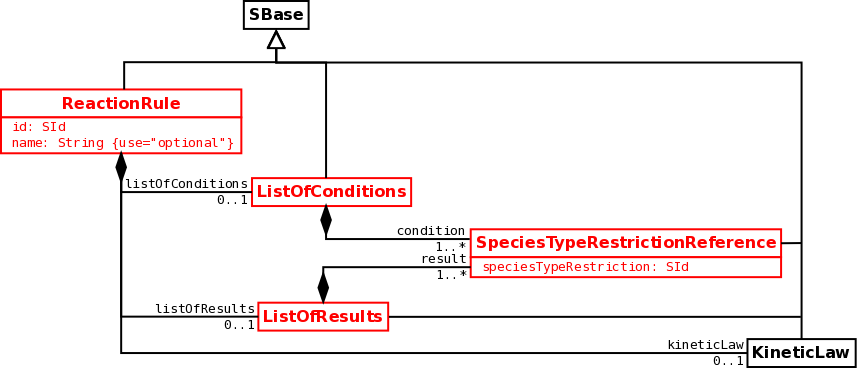
\includegraphics[scale=0.3]{./figs/pngs/ReactionRuleGeneral.png}
\caption{\class{ReactionRule} and all the associated classes of \multiVone.}
\end{center}
\end{figure}

\subsection{Reaction}

In order to encode the structures needed to propose alternative kinetic laws selected based on the state and connectivity of involved partners, we extend the element \class{Reaction} of \sbmlLthreeVone core by linking it to a list of \class{ReactionRule}s.

\begin{figure}[H]
\begin{center}
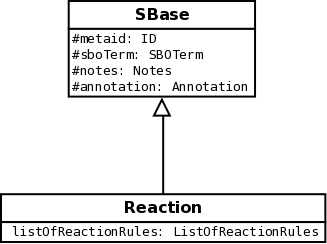
\includegraphics[scale=0.3]{figs/pngs/ReactionClass.png} 
\caption{Definition of the extended version of \class{Reaction} and its relation with \class{SBase}.}
\label{fig:ReactionClass}
\end{center}
\end{figure}

\begin{example}  
<reaction id="react" reversible="false" fast="false"
          xmlns:multi="http://www.sbml.org/sbml/level3/version1/multi/version1"> 
  <listOfReactants>
    <!-- some reactants -->
  </listOfReactants>
  <listOfProducts>
    <!-- some products -->
  <kineticLaw />
  <multi:listOfReactionRules>
    <!-- some reaction rules-->
  </multi:listOfReactionRules>
</reaction>
\end{example}

\subsection{SimpleSpeciesReference}

In order to decide which kinetic law to choose, one needs to have a list of the necessary states and connectivities for the partners involved. This is done by linking the \class{SimpleSpeciesReference} of \sbmlLthreeVone core to a list of \class{SpeciesTypeRestriction}s. There can be any number of \class{SpeciesTypeRestriction}s per \class{SimpleSpeciesReference}. They always represent alternatives, and only one can be used per \class{ReactionRule}. However, if one wants to discriminate between two instances of the same \class{Species} involved in the same \class{ReactionRule} but with different roles in the reaction, one must create two \class{SimpleSpeciesReference}s pointing to the same \class{Species}.

\begin{figure}[H]
\begin{center}
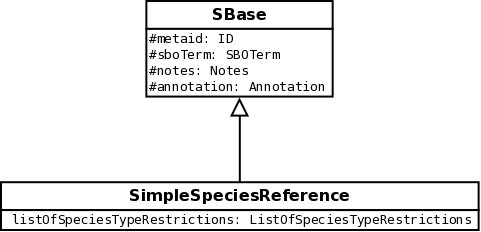
\includegraphics[scale=0.3]{figs/pngs/SimpleSpeciesReferenceClass.png} 
\caption{Definition of the extended version of \class{SimpleSpeciesReference} and its relation with \class{SBase}.}
\label{fig:SimpleSpeciesReferenceClass}
\end{center}
\end{figure}

\begin{example}
<speciesReference species="species1" stoichiometry="1"
                  xmlns:multi="http://www.sbml.org/sbml/level3/version1/multi/version1">
  <multi:listOfSpeciesTypeRestriction>
    <!-- some species type restrictions -->
  </multi:listOfSpeciesTypeRestriction>
</speciesReference>  
\end{example}

\subsection{ProductSpeciesReference}

In the cases where several instances of the same molecule are use in a reaction, we must explicit the correspondence between the reactants in the product. Otherwise, the following reactions will be selected by the same reaction rule:

\[A1-P + A2 \rightarrow A1 + A2-P\]

\[A1-P + A2 \rightarrow A1-P + A2\]

In order to do so, we create a new element \class{ProductSpeciesReference} that inherits from \class{SimpleSpeciesReference}. The element carries an attribute \attribute{correspondingReactant} that precises from which reactant instance the product originates. In an agent-based approach, this would apply to each 
molecule, while in a population-based framework, this would apply to pools. 

\begin{figure}[H]
\begin{center}
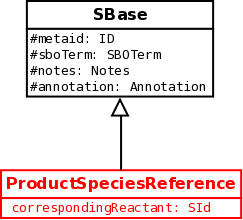
\includegraphics[scale=0.3]{figs/pngs/ProductSpeciesReferenceClass.png} 
\caption{Definition of the extended version of \class{ProductSpeciesReference} and its relation with \class{SBase}.}
\label{fig:ProductSpeciesReferenceClass}
\end{center}
\end{figure}

\begin{example}
<listOfReactants>
  <speciesReference id="R1" species="species1" stoichiometry="1"/>
  <speciesReference id="R2" species="species1" stoichiometry="1"/>
</listOfReactants>
<listOfProducts>
  <multi:productSpeciesReference species="species1" stoichiometry="1"
                xmlns:multi="http://www.sbml.org/sbml/level3/version1/multi/version1"
                multi:correspondingReactant="R1" />
  <multi:productSpeciesReference species="species1" stoichiometry="1"
                xmlns:multi="http://www.sbml.org/sbml/level3/version1/multi/version1"
                multi:correspondingReactant="R2" />
</listOfProducts>
\end{example}

\subsection{SpeciesTypeRestriction}

A \class{SpeciesTypeRestriction} points to a \class{SpeciesTypeInstances}, and creates a conditional species reference. Those various \class{SpeciesTypeRestriction}s can then be used to decide on the \class{ReactionRule} to use, and which \class{Result}s to produce. As all elements derived from \class{SBase}, it can link to \class{Notes} and \class{Annotation}, and carry a \attribute{metaid}, and an \attribute{sboTerm}.

\begin{figure}[H]
\begin{center}
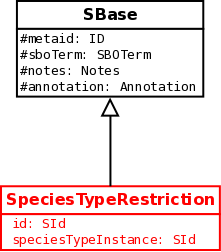
\includegraphics[scale=0.3]{figs/pngs/SpeciesTypeRestrictionClass.png} 
\caption{Definition of \class{SpeciesTypeRestriction} and its relation with \class{SBase}.}
\label{fig:SpeciesTypeRestrictionClass}
\end{center}
\end{figure}

\begin{example}
<multi:speciesTypeRestriction multi:id="speciesRest1" 
                   multi:speciesTypeInstance="speciesTypeInstance1" 
                   xmlns:multi="http://www.sbml.org/sbml/level3/version1/multi/version1"/>
\end{example}

\subsection{ReactionRule}

The \class{ReactionRule} element is used to describe a process that is dependent on states or connectivity. As all elements derived from \class{SBase}, it can link to \class{Notes} and \class{Annotation}, and carry a \attribute{metaid}, and an \attribute{sboTerm}. A \class{ReactionRule} applies when the conditions described in a \class{ListOfConditions} are fulfilled. The \class{ReactionRule} replaces the the regular \class{Reaction}. The effect of a \class{ReactionRule} is described by a \class{ListOfResults}. 

\begin{figure}[H]
\begin{center}
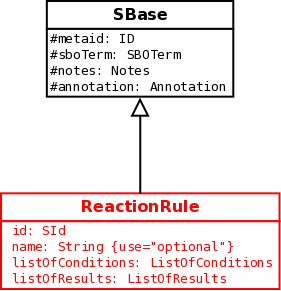
\includegraphics[scale=0.3]{figs/pngs/ReactionRuleClass.png} 
\caption{Definition of \class{ReactionRule} and its relation with \class{SBase}.}
\label{fig:ReactionRuleClass}
\end{center}
\end{figure}

\begin{example}
<multi:reactionRule multi:id="bindingNonPhospho"
         xmlns:multi="http://www.sbml.org/sbml/level3/version1/multi/version1" >
  <multi:listOfConditions>
    <!-- some conditions for the rule to be used-->
  </multi:listOfConditions>
  <multi:listOfResults>
    <!-- some results of the application of the rule -->
  </multi:listOfResults>
  <kineticLaw />
</multi:reactionRule>
\end{example}

\subsection{SpeciesTypeRestrictionReference}

In order to precise the conditions for a reaction rule to apply, and describe the results to obtain, a \class{SpeciesTypeRestrictionReference} points to a species type restriction using the attribute \attribute{speciesTypeRestriction}. As all elements derived from \class{SBase}, it can link to \class{Notes} and \class{Annotation}, and carry a \attribute{metaid}, and an \attribute{sboTerm}. The \class{SpeciesTypeRestriction}s used to decide if a rule applies are called in \class{ListOfConditions}. The \class{SpeciesTypeRestriction}s used to decide if the result of a rule are called in \class{ListOfResults}.

\begin{figure}[H]
\begin{center}
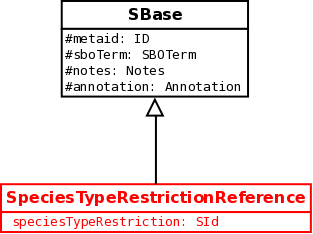
\includegraphics[scale=0.3]{figs/pngs/SpeciesTypeRestrictionReferenceClass.png} 
\caption{Definition of \class{SpeciesTypeRestrictionReference} and its relation with \class{SBase}.}
\label{fig:ConditionClass}
\end{center}
\end{figure}

\begin{example}
<multi:speciesTypeRestrictionReference multi:speciesTypeRestriction="freeRnonP"
          xmlns:multi="http://www.sbml.org/sbml/level3/version1/multi/version1" />
\end{example}

\subsection{ReactionRule -specific KineticLaw}

A \class{ReactionRule} optionally contains a \class{KineticLaw}. If the conditions apply, this \class{KineticLaw} is used to compute the results instead of the one contained in the reaction element of \sbmlLthreeVone. Note that the semantic of the model stripped of all information belonging to \multiVone may be understood in very different ways if the reaction does not contains a kineticLaw or contains an empty one. In the former case, stripping the species restrictions could means that the reaction always occurs, while in the latter, the reaction would have a flux of 0, effectively never happening. In the kinetic law of a reaction rule, the quantities of species are represented by the \attribute{id} of the \class{SpeciesTypeRestriction}s, and not the \attribute{id} of the  \class{Species}. This allows for multi-component reactions, where instances of the same species are playing different roles.

\subsection{Complete example of a reaction with reaction rules}

The following example describes a binding reaction that takes place ten times faster on the phosphorylated receptor than on the non-phosphorylated one.

\begin{example}
<reaction id="receptLigBinding" reversible="false" fast="false"> 
  <listOfReactants>
    <speciesReference id="spRef_Rec" species="receptor" stoichiometry="1">
      <multi:listOfSpeciesRestriction>
        <multi:speciesRestriction multi:id="restriction1" 
                                  multi:speciesTypeInstance="receptorNP" />
        <multi:speciesRestriction multi:id="restriction2"
                                  multi:speciesTypeInstance="receptorP" />
      </multi:listOfSpeciesRestriction>
    </speciesReference>
    <speciesReference species="ligand" stoichiometry="1" />
  </listOfReactants>
  <listOfProducts>
    <productSpeciesReference species="receptor" stoichiometry="1" 
                      correspondingReactant="spRef_Rec">
      <multi:listOfSpeciesRestriction>
        <multi:speciesRestriction multi:id="restriction3"
                                  multi:speciesTypeInstance="receptorBound" />
      </multi:listOfSpeciesRestriction>
    </productSpeciesReference>
  </listOfProducts>
  <kineticLaw>
    <math xmlns="http://www.w3.org/1998/Math/MathML" />
  </kineticLaw>
  <multi:listOfReactionRules>
    <multi:reactionRule multi:id="reactionRule1">
      <multi:listOfConditions>
        <multi:speciesTypeRestrictionReference multi:speciesTypeRestriction="restriction1"/>
      </multi:listOfConditions>
      <multi:listOfResults>
        <multi:speciesTypeRestrictionReference multi:speciesTypeRestriction="restriction3"/>
      </multi:listOfResults>
      <kineticLaw>
        <math xmlns="http://www.w3.org/1998/Math/MathML" >
          <ci> parameter1 </ci>
        </math>
        <listOfLocalParameters>
          <localParameter id="parameter1" value="1">
        </listOfLocalParameters>
      </kineticLaw>
    </multi:reactionRule>
    <multi:reactionRule multi:id="reactionRule2">
      <multi:listOfConditions>
        <multi:speciesTypeRestrictionReference multi:speciesTypeRestriction="restriction2"/>
      </multi:listOfConditions>
      <multi:listOfResults>
        <multi:speciesTypeRestrictionReference multi:speciesTypeRestriction="restriction3"/>
      </multi:listOfResults>
      <kineticLaw>
        <math xmlns="http://www.w3.org/1998/Math/MathML" >
          <ci> parameter2 </ci>
        </math>
        <listOfLocalParameters>
          <localParameter id="parameter2" value="10">
        </listOfLocalParameters>
      </kineticLaw>
    </multi:reactionRule>
  </multi:listOfReactionRules>
</reaction>
\end{example}

\section{Assignments following discrete events}

In \sbmlLthreeVone, \class{EventAssignment}s are used to assign values to variables of a model, that are \class{Compartment}s, \class{Species}, \class{SpeciesReference}, or global \class{Parameter}s  when some conditions are fulfilled. In order to assign the value of a specific type of species, \class{EventAssignment}s in \multiVone also contain an element \class{SpeciesTypeInstanceChange}. The assignment sets the quantity of instances that fulfil a certain selection using the mathematical expression provided. 

\begin{figure}[h!]
\begin{center}
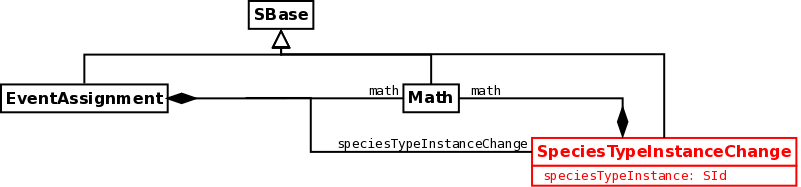
\includegraphics[scale=0.3]{./figs/pngs/EventAssignmentGeneral.png}
\caption{\class{EventAssignment} and all the associated classes of \multiVone.}
\end{center}
\end{figure}

\subsection{EventAssignment}

In order to assign values to entity subpools, defined by specific state and connectivity, following a discrete event, the element \class{eventAssignment} of \sbmlLthreeVone core is linked to a \class{SpeciesTypeInstanceChange}.

\begin{figure}[H]
\begin{center}
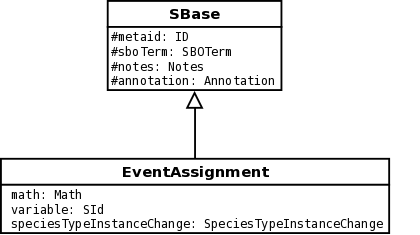
\includegraphics[scale=0.4]{figs/pngs/EventAssignmentClass.png} 
\caption{Definition of the extended version of \class{EventAssignment} and its relation with \class{SBase}.}
\label{fig:EventAssignmentClass}
\end{center}
\end{figure}

\subsection{SpeciesTypeInstanceChange}

For a definition of \class{SpeciesTypeInstanceChange}, see section \ref{SpeciesTypeInstanceChange}.